\date{}
\title{}
\date{}
\begin{document}


\begin{frame}
    \titlepage
\end{frame}

\begin{frame}{last time}
    \begin{itemize}
    \item string instructions
    \item thread-local storage through segmentation hack
    \item ELF-format executables/object files
    \item sections / segments
    \item LOAD directives
    \end{itemize}
\end{frame}


\makeatletter
\newenvironment<>{btHighlight}[1][]
{\begin{onlyenv}#2\begingroup\tikzset{bt@Highlight@par/.style={#1}}\begin{lrbox}{\@tempboxa}}
{\end{lrbox}\bt@HL@box[bt@Highlight@par]{\@tempboxa}\endgroup\end{onlyenv}}

\newcommand<>\btHL[1][]{%
  \only#2{\begin{btHighlight}[#1]\bgroup\aftergroup\bt@HL@endenv}%
}
\def\bt@HL@endenv{%
  \end{btHighlight}%   
  \egroup %
}
\tikzset{
    btHLbox/.style={
        fill=red!30,outer sep=0pt,inner xsep=1pt, inner ysep=0pt, rounded corners=3pt
    },
}
\newcommand{\bt@HL@box}[2][]{%
  \tikz[#1]{%
    \pgfpathrectangle{\pgfpoint{1pt}{0pt}}{\pgfpoint{\wd #2}{\ht #2}}%
    \pgfusepath{use as bounding box}%
    \node[text width={},draw=none,anchor=base west, btHLbox, minimum height=\ht\strutbox+1pt,#1]{\raisebox{1pt}{\strut}\strut\usebox{#2}};
  }%
}

\lst@CCPutMacro
    \lst@ProcessOther {"2A}{%
      \lst@ttfamily 
         {\raisebox{2pt}{*}}% used with ttfamily
         {\raisebox{2pt}{*}}}% used with other fonts
    \@empty\z@\@empty

\lstdefinelanguage
   [x8664gas]{Assembler}     % add a "x64" dialect of Assembler
   [x86masm]{Assembler} % based on the "x86masm" dialect
   % with these extra keywords:
   {morekeywords={CDQE,CQO,CMPSQ,CMPXCHG16B,JRCXZ,LODSQ,MOVSXD,%
                  POPFQ,PUSHFQ,SCASQ,STOSQ,IRETQ,RDTSCP,SWAPGS,.TEXT,.STRING,.ASCIZ,%
                  BEQ,LW,SW,LB,SB,ADDIU,J,BEQZ,BNEZ,BNE,%
                  MOVUPD,MULPD,MOVSD,MULSD,%
                  SHLADD,MOV,CMP.LT,TBIT.NZ,BR.RET.SPTK.MANY,%
                  ADDQ,POPQ,PUSHQ,RRMOVQ,MRMOVQ,RMMOVQ,IRMOVQ,%
                  <-,LL,SC,ADDI,ADDL,VMOVDQA,ADDQ,CMPL,JB,JBE,MOVL,CLTQ,%
                  MOVW,PUSHW,MOV,ADD,SUB,INT,PUSH,MOV,ADD,REP,MOVSB,%
                  TESTQ,CMPQ,MOVL,MOVQ,ADDQ,JMPQ,XORQ,%
                  LEAQ,LEAL,LEA,RETQ,RET,POPL,POPW,PUSHL,PUSHW,%
                  LEAW,%
                  SUBQ,SYSCALL,.ASCII,CALLQ,MOVSLQ,JMP,ANDQ,SHRQ,MOVB,INCQ,TESTL,XORL,%
                  SHRL,LEAL,SARL,SUBL,IMULL,IMULQ,MOVDQU,PADDD,XORL,%
                  MOVZBL,MOVZB,SHRB,SRAL,SHRL,ANDL,%
                  CMOVNS,SRAL,SRAQ,MOVZBW,MOVZBQ,%
                  PADDW,PADDQ,MODUPS,MOVAPD,%
                  MOVL,RET,.GLOBL,%
		  PAUSE,LFENCE,JMP,%
                  },
    deletekeywords={eax,ebx,sp,si,cx,di,ds,cs,es,fs,dx,ax,bx,al,esi,ebp,ecx,rip,eip,edx,edi,rdi,esp},
    deletekeywords=[2]{size},
    alsoletter={\%},
    alsoother={()},
    emphstyle={\color{violet!50!black}},
    emph={\%rax,\%rbx,\%rcx,\%rdx,\%r8,\%r9,\%r10,\%r11,\%r12,\%r13,\%r14,\%r15,\%eax,\%ebx,\%sp,\%si,\%cx,\%di,\%ds,\%cs,\%es,\%fs,\%dx,\%ax,\%bx,\%al,\%esi,\%ebp,\%ecx,\%rip,\%eip,\%edx,\%edi,\%rdi,\%esp,\%rsp},
    %moreemph={eax,ebx,sp,si,cx,di,ds,cs,es,fs,dx,ax,bx,al,esi,ebp,ecx,rip,eip,edx,edi,rdi,esp},
    morecomment=[l]{\#},
    morecomment=[l]{\/\/},
    morecomment=[s]{/*}{*/},
    sensitive=false,
    keepspaces=true} % et

\lstalias[]{myasm}[x8664gas]{Assembler}

\lstdefinelanguage{JavaScript}{
  keywords={typeof, new, true, false, catch, function, return, null, catch, switch, var, if, in, while, do, else, case, break},
  ndkeywords={class, export, boolean, throw, implements, import, this},
  sensitive=false,
  comment=[l]{//},
  morecomment=[s]{/*}{*/},
  morestring=[b]',
  morestring=[b]"
}

\newcommand{\keywordstyle}{\sourcecodeprolight\bfseries\color{blue!30!black}}
\newcommand{\stringstyle}{\color{blue!20!black}\ttfamily}

\lstset{
    language=C,
    basicstyle=\sourcecodepro\EmptyMapping,
    escapechar=`,
    keywordstyle=\keywordstyle\EmptyMapping,
    identifierstyle=\sourcecodepro\EmptyMapping,
    numberstyle=\small\color{black!70},
    commentstyle=\color{red!60!black}\ttfamily\itshape,
    stringstyle=\color{blue!20!black}\ttfamily,
    ndkeywordstyle=\bfseries\color{blue!30!black},
    upquote=true,
}



\lstdefinestyle{medium}{
    basicstyle=\sourcecodepro\EmptyMapping\fontsize{12}{13}\selectfont,
    keywordstyle=\sourcecodepro\EmptyMapping\fontsize{12}{13}\selectfont\keywordstyle,
}

\lstdefinestyle{small}{
    basicstyle=\sourcecodepro\EmptyMapping\small,
    keywordstyle=\sourcecodepro\EmptyMapping\small\keywordstyle,
}

\lstdefinestyle{smaller}{
    basicstyle=\sourcecodepro\EmptyMapping\fontsize{11}{12}\selectfont,
    keywordstyle=\sourcecodepro\EmptyMapping\fontsize{11}{12}\selectfont\keywordstyle,
}

\lstdefinestyle{size105}{
    basicstyle=\sourcecodepro\EmptyMapping\fontsize{10.5}{11.5}\selectfont,
    keywordstyle=\sourcecodepro\EmptyMapping\fontsize{10.5}{11.5}\selectfont\keywordstyle,
}

\lstdefinestyle{size10}{
    basicstyle=\sourcecodepro\EmptyMapping\fontsize{10}{11}\selectfont,
    keywordstyle=\sourcecodepro\EmptyMapping\fontsize{10}{11}\selectfont\keywordstyle,
}

\lstdefinestyle{size9}{
    basicstyle=\sourcecodepro\EmptyMapping\fontsize{9}{10}\selectfont,
    keywordstyle=\sourcecodepro\EmptyMapping\fontsize{9}{10}\selectfont\keywordstyle,
}
\lstdefinestyle{size8}{
    basicstyle=\sourcecodepro\EmptyMapping\fontsize{8}{9}\selectfont,
    keywordstyle=\sourcecodepro\EmptyMapping\fontsize{8}{9}\selectfont\keywordstyle,
}



\lstdefinestyle{script}{
    basicstyle=\sourcecodepro\EmptyMapping\scriptsize,
    keywordstyle=\sourcecodepro\EmptyMapping\scriptsize\bfseries,
}




\subsection{program headers: example static ELF binary}

\providecommand{\myemphTwo}[1]{\myemph<2>{#1}}
\providecommand{\myemphTwoB}[1]{\myemph<2>{\textbf<2>{#1}}}
\providecommand{\myemphThree}[1]{\myemph<3>{#1}}
\providecommand{\myemphFour}[1]{\myemph<4>{#1}}
\providecommand{\myemphFive}[1]{\myemph<5>{#1}}
\providecommand{\myemphSix}[1]{\myemph<6>{#1}}
\providecommand{\myemphSeven}[1]{\myemph<7>{#1}}

\begin{frame}[fragile,label=elfExOver1]{ELF example}
    \begin{itemize}
    \item {\tt objdump -x /bin/busybox} (on my laptop)
    \item {\tt -x}: output all headers
    \end{itemize}
\begin{Verbatim}[commandchars=\\\{\},fontsize=\small]
/bin/busybox:     file format \myemphTwo{elf64-x86-64}
/bin/busybox
architecture: i386:x86-64, flags 0x00000102:
EXEC_P, D_PAGED
start address \myemphThree{0x0000000000402170}

Program Header:
[...]

Sections:
[...]
\end{Verbatim}
\end{frame}

\begin{frame}[fragile,label=elfExOver2]{a program header (1)}
\begin{Verbatim}[commandchars=\\\{\},fontsize=\fontsize{9}{10}\selectfont]
Program Header:
[...]
LOAD off    0x0001000 vaddr 0x0401000 paddr 0x0401000 align 2**12
     filesz \myemphTwo{0x01b04ed} memsz 0x01b04ed flags \myemphThree{r-x}
[...]
LOAD off    0x0207950 vaddr 0x0608950 paddr 0x0608950 align 2**12
     filesz \myemphFour{0x0008f40} memsz \myemphFour{0x000c718} flags rw-

\end{Verbatim}
\begin{itemize}
\item load {\tt \myemph<2>{0x1bd04ed}} bytes:
        \begin{itemize}
        \item from {\tt 0x1000} bytes into the file 
        \item to memory at {\tt 0x401000} \\
        \item \myemph<3>{readable and executable}
        \end{itemize}
\item load {\tt 0x8f40} bytes:
        \begin{itemize}
        \item from {\tt 0x207950} bytes into the file 
        \item to memory at {\tt 0x608950} 
        \item \myemph<4>{plus ({\tt 0xc718}--{\tt 0x8f40}) bytes of zeroes}
        \item readable and writable
        \end{itemize}
\end{itemize}
\end{frame}

\begin{frame}[fragile,label=elfExOver3]{a program header (2)}
\begin{Verbatim}[commandchars=\\\{\},fontsize=\fontsize{9}{10}\selectfont]
Program Header:
[...]
    NOTE off    0x0000290 vaddr 0x0400290 paddr 0x0400290 align 2**2
         filesz 0x0000044 memsz 0x0000044 flags r--
     TLS off    0x0207950 vaddr 0x0608950 paddr 0x0608950 align 2**3
         filesz 0x0000030 memsz 0x0000092 flags r--
0x6474e553 off  0x0000270 vaddr 0x0400270 paddr 0x0400270 align 2**3
         filesz 0x0000020 memsz 0x0000020 flags r--
   STACK off    0x0000000 vaddr 0x0000000 paddr 0x0000000 align 2**4
         filesz 0x0000000 memsz 0x0000000 flags rw-
   RELRO off    0x0207950 vaddr 0x0608950 paddr 0x0608950 align 2**0
         filesz 0x00066b0 memsz 0x00066b0 flags r--
[...]
\end{Verbatim}
\begin{itemize}
\item NOTE --- comment
\item TLS --- thread-local storage region (used via {\tt \%fs})
\item 0x6474e553 --- `GNU\_PROPERTY' --- adtl linker/loader info
\item STACK --- indicates stack is read/write
\item RELRO --- make this read-only after runtime linking
\end{itemize}
\end{frame}




\subsection{ELF LOAD}
\usetikzlibrary{arrows.meta,decorations.pathmorphing,patterns}

\begin{frame}<2->{ELF LOAD}
\begin{tikzpicture}
\begin{pgfonlayer}{fg}
    \draw[very thick] (0, 0) rectangle (4, 6);
\node[font=\huge,black!25,align=center] at (2, 3) {
    program \\ on\\ disk
};
\end{pgfonlayer}
\coordinate (header tl) at (4, 0.5);
\coordinate (header br) at (0, 0);
\coordinate (load off) at (0, 1);
\coordinate (load end) at (0, 2.54);
\draw[thick,Latex-,font=\small] (0, 0) -- ++(-.5, 0) node[left,align=right] {off {\tt 0}\\ (start)};

\begin{scope}[xshift=6cm]
    \begin{pgfonlayer}{fg}
        \draw[very thick] (0, 7) -- (0, 0) -- (4, 0) -- (4, 7);
        \draw[overlay,very thick,decorate,decoration={zigzag,segment length=2.5mm}] (0, 7) -- (4, 7);
    \node[font=\huge,black!25,align=center] at (2, 3) {
        program \\ in\\ memory
    };
    \end{pgfonlayer}
    \coordinate (vaddr off) at (4, 4);
    \coordinate (vaddr end copy) at (4, 5.54);
    \coordinate (vaddr end all) at (4, 6.64);
\draw[thick,Latex-,font=\small] (4, 0) -- ++(.5, 0) node[right,align=left] {addr {\tt 0}};
\end{scope}
\begin{visibleenv}<2->
    \fill[blue!30] (header tl) rectangle (header br);
    \node[align=left,font=\small\tt,anchor=north west,draw] (load) at (1, -.25) {
        LOAD off {\color{green!50!black}0x1000} vaddr {\color{violet!70}0x4000} \ldots \\
        \hspace{1cm} filesz 0x1544 memsz 0x2644 \ldots
    };
    \draw[dotted,thick] ([yshift=-1mm]header tl -| header br) -- (load.north west);
    \draw[dotted,thick] ([xshift=3cm,yshift=-1mm]header tl -| header br) -- (load.north east);
\end{visibleenv}
\begin{visibleenv}<3->
    \draw[very thick,Latex-] (load off) -- ++(-.5cm,0) node[left,font=\small] {{\color{green!50!black}\tt 0x1000}};
    \draw[very thick,Latex-] (vaddr off) -- ++ (.5cm, 0) node[right,font=\small] {{\color{violet!70}\tt 0x4000}};
    \draw[thick,Latex-Latex] ([xshift=-.15cm]load off) -- ([xshift=-.15cm]load end)
        node[midway,font=\small,left] {\tt 0x1544};
    \draw[thick,Latex-Latex] ([xshift=.15cm]vaddr off) -- ([xshift=.15cm]vaddr end copy)
        node[midway,font=\small,right] {\tt 0x1544};
    \draw[thick,Latex-Latex] ([xshift=-4.15cm]vaddr off) -- ([xshift=-4.15cm]vaddr end all)
        node[midway,font=\small,left] {\tt 0x2644};
    \fill[red!20] (load off) rectangle ([xshift=4cm]load end);
    \fill[red!20] (vaddr off) rectangle ([xshift=-4cm]vaddr end copy);
    \fill[pattern=north west lines] (vaddr end copy) rectangle ([xshift=-4cm]vaddr end all);
\end{visibleenv}
\end{tikzpicture}
\end{frame}


\subsection{position independent executables}

\providecommand{\myemphA}[1]{\myemph<1>{#1}}
\providecommand{\myemphB}[1]{\myemph<2>{#1}}
\begin{frame}[fragile,label=dl-libs]{dynamic library headers}
\begin{Verbatim}[commandchars=\\\{\},fontsize=\fontsize{9}{10}\selectfont]
/lib/x86_64-linux-gnu/libc.so.6:     file format elf64-x86-64
/lib/x86_64-linux-gnu/libc.so.6
architecture: i386:x86-64, flags 0x00000150:
HAS_SYMS, \myemphA{DYNAMIC}, D_PAGED
start address 0x00000000000271f0

Program Header:
    PHDR off    0x0000000000000040 vaddr 0x0000000000000040 paddr 0x0000000000000040 align 2**3
         filesz 0x0000000000000310 memsz 0x0000000000000310 flags r--
  INTERP off    0x00000000001c16a0 vaddr 0x00000000001c16a0 paddr 0x00000000001c16a0 align 2**4
         filesz 0x000000000000001c memsz 0x000000000000001c flags r--
    LOAD off    0x0000000000000000 vaddr \myemphB{0x0000000000000000} paddr 0x0000000000000000 align 2**12
         filesz 0x0000000000024940 memsz 0x0000000000024940 flags r--
...
\end{Verbatim}
\begin{tikzpicture}[overlay,remember picture]
\begin{visibleenv}<1>
\node[draw,very thick,anchor=south] at ([yshift=.5cm]current page.south) {
    DYNAMIC --- instead of EXEC\_P
};
\end{visibleenv}
\begin{visibleenv}<2>
\node[draw,very thick,anchor=south,align=left] at ([yshift=.5cm]current page.south) {
    specifies loading starting at address 0 \\
    but dynamic linker will actually choose a different starting address
};
\end{visibleenv}
\end{tikzpicture}
\end{frame}

\begin{frame}[fragile,label=pie-headers]{position-independent executables}
\begin{Verbatim}[commandchars=\\\{\},fontsize=\fontsize{9}{10}\selectfont]
hello.exe:     file format elf64-x86-64
hello.exe
architecture: i386:x86-64, flags 0x00000150:
HAS_SYMS, \myemphA{DYNAMIC}, D_PAGED
start address 0x0000000000001080

Program Header:
    PHDR off    0x0000000000000040 vaddr 0x0000000000000040 paddr 0x0000000000000040 align 2**3
         filesz 0x00000000000002d8 memsz 0x00000000000002d8 flags r--
  INTERP off    0x0000000000000318 vaddr 0x0000000000000318 paddr 0x0000000000000318 align 2**0
         filesz 0x000000000000001c memsz 0x000000000000001c flags r--
    LOAD off    0x0000000000000000 vaddr \myemphB{0x0000000000000000} paddr 0x0000000000000000 align 2**12
         filesz 0x00000000000005f8 memsz 0x00000000000005f8 flags r--
\end{Verbatim}
\begin{tikzpicture}[overlay,remember picture]
\begin{visibleenv}<1>
\node[draw,very thick,anchor=south,align=left] at ([yshift=.5cm]current page.south) {
    executable with headers like dynamic library \\
    ``position-independent executable'': can be loaded at any address
};
\end{visibleenv}
\end{tikzpicture}
\end{frame}


\section{aside: other formats}


\begin{frame}{other executable formats}
    \begin{itemize}
    \item PE (Portable Executable) --- Windows
    \item Mach-O --- MacOS X
    \item broadly similar to ELF
    \item differences:  
        \begin{itemize}
        \item whether segment/section distinction exists
        \item how linking/debugging info represented
        \item how program start info represented
        \end{itemize}
    \end{itemize}
\end{frame}




\section{executable startup} % FIXME: shorten?


\begin{frame}{simple executable startup}
    \begin{itemize}
    \item copy segments into memory
    \item jump to start address
    \end{itemize}
\end{frame}

\begin{frame}{executable startup code}
    \begin{itemize}
    \item Linux: executables don't start at {\tt main}
    \item why not?
        \begin{itemize}
        \item need to initialize {\tt printf}, {\tt cout}, {\tt malloc}, etc. data structures
        \item {\tt main} needs to return somewhere
        \end{itemize}
    \item compiler links in startup code
    \end{itemize}
\end{frame}




\section{dynamic linking}

\subsection{linking primer}

\usetikzlibrary{positioning}
\begin{frame}{linking}
    \begin{tikzpicture}
    \node[draw,font=\tt,very thick] (theCall) {callq printf};
    \node[draw,font=\tt,below=5cm of theCall,very thick] (theCallResolved) {callq 0x458F0};
    \draw[very thick,-Latex] (theCall) -- (theCallResolved);
    \end{tikzpicture}
\end{frame}

\begin{frame}{static v. dynamic linking}
    \begin{itemize}
    \item static linking --- linking \myemph{to create executable}
    \item dynamic linking --- linking \myemph{when executable is run}
    \vspace{.5cm}
    \item<2> conceptually: no difference in how they work
    \item<2> reality --- very different mechanisms
    \end{itemize}
\end{frame}

\begin{frame}{linking data structures}
    \begin{itemize}
    \item symbol table: {\tt name} $\Rightarrow$ (section, offset)
        \begin{itemize}
        \item example: {\tt main:} in assembly adds symbol table entry for {\tt main}
        \end{itemize}
    \item relocation table: offset $\Rightarrow$ (name, kind)
        \begin{itemize}
        \item example: {\tt call printf} adds relocation for name {\tt printf}
        \item kind depends on how instruction encodes address
        \end{itemize}
    \end{itemize}
\end{frame}

 % FIXME: change to have executable version

\subsubsection{in objdump, static}
\begin{frame}[fragile,label=linkingExAsm]{hello.s}
\begin{lstlisting}
.data
string: .asciz "Hello, World!"
.text
.globl main
main:
    movq $string, %rdi
    call puts
    ret
\end{lstlisting}
\end{frame}

\begin{frame}[fragile,label=linkingExObjRepeat]{hello.o (pre-static or dynamic linking)}
\begin{Verbatim}[commandchars=\\\{\},fontsize=\fontsize{9}{10}\selectfont]
SYMBOL TABLE:
0000000000000000 l    d  .text  0000000000000000 .text
0000000000000000 l    d  .data  0000000000000000 .data
0000000000000000 l    d  .bss   0000000000000000 .bss
0000000000000000 l       .data  0000000000000000 string
0000000000000000 \myemphSix{g}       \myemphSeven{.text  0000000000000000} main
0000000000000000         \myemphTwo{*UND*  0000000000000000 puts}

RELOCATION RECORDS FOR [.text]:
OFFSET           TYPE              VALUE 
0000000000000003 \myemphFive{R_X86_64_32S}      \myemphFour{.data}
0000000000000008 \myemphFive{R_X86_64_PC32}     \myemphThree{puts}-0x0000000000000004
\end{Verbatim}
\begin{tikzpicture}[overlay,remember picture]
    \tikzset{overBox/.style={at=(boxLoc),anchor=center,align=center,draw,rectangle,fill=white}}
    \coordinate (boxLoc) at ([yshift=-2.5cm]current page.center);
    \begin{visibleenv}<2>
        \node[overBox] {
            undefined symbol: look for {\tt puts} elsewhere
        };
    \end{visibleenv}
    \begin{visibleenv}<3>
        \node[overBox] {
           insert address of puts, format for {\tt call}
        };
    \end{visibleenv}
    \begin{visibleenv}<4>
        \node[overBox] {
           insert address of string, format for {\tt movq}
        };
    \end{visibleenv}
    \begin{visibleenv}<5>
        \node[overBox] {
            different ways to represent address \\
            {\tt 32S} --- signed 32-bit value \\
            {\tt PC32} --- 32-bit difference from current address
        };
    \end{visibleenv}
    \begin{visibleenv}<6>
        \node[overBox] {
            {\tt g}: global --- used by other files \\
            {\tt l}: local 
        };
    \end{visibleenv}
    \begin{visibleenv}<7>
        \node[overBox] {
            {\tt .text} segment beginning plus 0 bytes
        };
    \end{visibleenv}
\end{tikzpicture}
\end{frame}

\begin{frame}[fragile]{hello.o / statically linked, no PIE}
hello.o:
\begin{Verbatim}[commandchars=\\\{\},fontsize=\fontsize{9}{10}\selectfont]
Disassembly of section .text:

0000000000000000 <main>:
   0:   48 c7 c7 00 00 00 00    mov    $0x0,%rdi
                        3: R_X86_64_32S .data
   7:   e8 00 00 00 00          call   c <main+0xc>
                        8: R_X86_64_PLT32       puts-0x4
   c:   c3                      ret    
\end{Verbatim}
\hrule
hello.exe (gcc -static -no-pie):
\begin{Verbatim}[commandchars=\\\{\},fontsize=\fontsize{9}{10}\selectfont]
Disassembly of section .text:
...
 00000000004016c3 <main>:
   4016c3:▶      48 c7 c7 b5 16 40 00 ▶  mov    $0x4016b5,%rdi
   4016ca:▶      e8 e1 a9 00 00       ▶  call   40c0b0 <_IO_puts>
   4016cf:▶      c3                   ▶  ret    
...
\end{Verbatim}
\end{frame}



\subsection{aside: symbols in statically linked helo}
\begin{frame}[fragile]{symbols in executable}
\begin{Verbatim}[fontsize=\small]
SYMBOL TABLE:
0000000000000000 l    df *ABS*  0000000000000000 crt1.o
00000000004002b4 l     O .note.ABI-tag  0000000000000020 __abi_tag
0000000000000000 l    df *ABS*  0000000000000000 assert.o
0000000000498530 l     O .rodata        0000000000000013 errstr.0
0000000000401100 l     F .text  000000000000000f __assert_fail_base.cold
\end{Verbatim}
\ldots
\begin{itemize}
\item by default, symbol information in statically-linked executable
\item \ldots but not actually used to run it!
\vspace{.5cm}
\item can be stripped (-s linker option or strip command) isntead:
\end{itemize}
\begin{Verbatim}[fontsize=\small]
SYMBOL TABLE:
no symbols
\end{Verbatim}
\end{frame}

\begin{frame}{exercise: finding without symbols?}
\begin{itemize}
\item how can I find where functions are without symbols?
\item ideally: some \textit{automated} way to do this?
\end{itemize}
\end{frame}


\subsection{aside: strace, statically linked strace}
\begin{frame}{interlude: strace}
\begin{itemize}
\item {\tt strace} --- system call tracer
    \begin{itemize}
    \item on Linux, some other Unices
    \item OS X approx. equivalent: {\tt dtruss}
    \item Windows approx. equivalent: Process Monitor
    \end{itemize}
\item indicates what system calls (operating system services) used by a program
\end{itemize}
\end{frame}

\begin{frame}[fragile,label=staticStrace]{statically linked hello.exe}
\begin{itemize}
\item \small{\tt gcc -no-pie -static -o hello-static.exe hello.s}
\item \small{\tt strace ./hello-static.exe}:
\end{itemize}
\begin{Verbatim}[commandchars=@\{\},fontsize=\fontsize{8}{9}\selectfont]
execve("./hello-static.exe", ["./hello-static.exe"], [/* 46 vars */]) = 0
@myemphTwo{uname({sysname="Linux", nodename="reiss-lenovo", ...}) = 0}
@myemphTwo{brk(NULL)                               = 0x20a5000}
@myemphThree{brk(0x20a61c0)                          = 0x20a61c0}
@myemphTwo{arch_prctl(ARCH_SET_FS, 0x20a5880)      = 0}
@myemphTwo{readlink("/proc/self/exe", "/home/cr4bd/spring2017/cs4630/sl"..., 4096) = 62}
@myemphThree{brk(0x20c71c0)                          = 0x20c71c0}
@myemphThree{brk(0x20c8000)                          = 0x20c8000}
@myemphTwo{access("/etc/ld.so.nohwcap", F_OK)}      = -1 ENOENT (No such file or directory)
@myemphFour{fstat(1, {st_mode=S_IFCHR|0620, st_rdev=makedev(136, 1), ...}) = 0}
@myemphFour{write(1, "Hello, World!\n", 14)         = 14}
@myemphFive{exit_group(14)}                          = ?
+++ exited with 14 +++
\end{Verbatim}
\begin{tikzpicture}[overlay,remember picture]
    \tikzset{
        overBoxGeneric/.style={
            anchor=center,
            align=center,
            draw,
            rectangle,
            fill=white,
            draw=red!70!black,very thick},
        overBox/.style={
            overBoxGeneric,
            at=(boxLoc),
        },
        overBoxB/.style={
            overBoxGeneric,
            at=(boxLocB),
        },
    }
    \coordinate (boxLoc) at ([yshift=-3.5cm]current page.center);
    \begin{visibleenv}<2>
        \node[overBox] {
            standard library startup
        };
    \end{visibleenv}
    \begin{visibleenv}<3>
        \node[overBox] {
            memory allocation
        };
    \end{visibleenv}
    \begin{visibleenv}<4>
        \node[overBox] {
            implementation of puts
        };
    \end{visibleenv}
    \begin{visibleenv}<5>
        \node[overBox] {
            standard library shutdown
        };
    \end{visibleenv}
\end{tikzpicture}
\end{frame}



\subsection{example: strace hello.exe dynamic}

\begin{frame}[fragile,label=straceDynamic]{dynamically linked hello.exe}
\begin{itemize}
\item \small{\tt gcc -o hello.exe hello.s}
\item \small{\tt strace ./hello.exe}:
\end{itemize}
\begin{Verbatim}[commandchars=@\{\},fontsize=\fontsize{8}{9}\selectfont]
execve("./hello.exe", ["./hello.exe"], [/* 46 vars */]) = 0
@textit{...}
@myemphThree{mmap(NULL, 8192, PROT_READ|PROT_WRITE, MAP_PRIVATE|MAP_ANONYMOUS, -1, 0)} = 0x7fdfeeb39000
access("/etc/ld.so.preload", R_OK)      = -1 ENOENT (No such file or directory)
open("/etc/ld.so.cache", O_RDONLY|O_CLOEXEC) = 3
fstat(3, {st_mode=S_IFREG|0644, st_size=137808, ...}) = 0
@textit{...}
open("@myemphTwoB{/lib/x86_64-linux-gnu/libc.so.6}", O_RDONLY|O_CLOEXEC) = 3
@myemphFour{read(3, "\177ELF\2\1\1\3\0\0\0\0\0\0\0\0\3\0>\0\1\0\0\0P\t\2\0\0\0\0\0"..., 832) = 832}
fstat(3, {st_mode=S_IFREG|0755, st_size=1864888, ...}) = 0
@myemphFive{mmap(NULL, 3967392, PROT_READ|PROT_EXEC, ..., 3, 0) = 0x7fdfee54d000}
mprotect(0x7fdfee70c000, 2097152, PROT_NONE) = 0
@myemphFive{mmap(0x7fdfee90c000, 24576, PROT_READ|PROT_WRITE, ..., 3, 0x1bf000) = 0x7fdfee90c000}
@myemphSix{mmap(0x7fdfee912000, 14752, PROT_READ|PROT_WRITE, ..., -1, 0) = 0x7fdfee912000}
close(3)                                = 0
@textit{...}
write(1, "Hello, World!\n", 14)         = 14
exit_group(14)                          = ?
+++ exited with 14 +++
\end{Verbatim}
\begin{tikzpicture}[overlay,remember picture]
    \tikzset{overBox/.style={at=(boxLoc),anchor=center,align=center,draw,rectangle,fill=white,draw=red!70!black,very thick}}
    \coordinate (boxLoc) at ([yshift=-2cm]current page.center);
    \begin{visibleenv}<2>
        \node[overBox] {
            the standard C library (includes {\texttt{puts}})
        };
    \end{visibleenv}
    \begin{visibleenv}<3>
        \node[overBox] {
            memory allocation (different method)
        };
    \end{visibleenv}
    \begin{visibleenv}<4>
        \node[overBox] {
            read standard C library header
        };
    \end{visibleenv}
    \begin{visibleenv}<5>
        \node[overBox] {
            load standard C library ({\tt 3} = opened file)
        };
    \end{visibleenv}
    \begin{visibleenv}<6>
        \node[overBox] {
            allocate zero-initialized data segment for C library
        };
    \end{visibleenv}
\end{tikzpicture}
\end{frame}



\subsection{where's the linker}


\begin{frame}{where's the linker}
\begin{itemize}
    \item Where's the code that calls {\tt open("...libc.so.6")}?
    \item Could check {\tt hello.exe} --- it's not there!
    \vspace{.5cm}
    \item<2> instead: ``interpreter'' {\tt /lib64/ld-linux-x86-64.so.2}
    \item<2> on Linux: contains loading code instead of core OS
        \begin{itemize}
        \item OS loads it instead of program
        \end{itemize}
\end{itemize}
\end{frame}

\begin{frame}[fragile,label=interpObjdump]{objdump --- the interpreter}
\begin{itemize}
\item excerpt from {\tt objdump -sx hello.exe}:
\end{itemize}
\begin{Verbatim}[commandchars=@\{\},fontsize=\fontsize{8}{9}\selectfont]
Program Header:
@textit{...}
  INTERP off    0x0000238 vaddr 0x0@myemph{400318} paddr 0x0400238 align 2**0
         filesz 0x000001c memsz 0x000001c flags r--
@textit{...}
Contents of section .interp:
 @myemph{400318} 2f6c6962 36342f6c 642d6c69 6e75782d  @myemph{/lib64/ld-linux-}
 400328 7838362d 36342e73 6f2e3200           @myemph{x86-64.so.2}.    
\end{Verbatim}
\end{frame}


\subsection{knowing what to load?}

\begin{frame}[fragile,label=dynLinkNeeded1]{dynamic linking: what to load? (1)}
\begin{itemize}
\item excerpt from {\tt objdump -sx hello.exe}:
\end{itemize}
\begin{Verbatim}[commandchars=@\{\},fontsize=\fontsize{9}{10}\selectfont]
Program Header:
@textit{...}
 @myemph{DYNAMIC} off    0x0000000000002e20 vaddr 0x0000000000403e20 paddr 0x0000000000403e20 align 2**3
         filesz 0x00000000000001d0 memsz 0x00000000000001d0 flags rw-
@textit{...}
Dynamic Section:
  @myemph{NEEDED               libc.so.6}
  INIT                 0x0000000000401000
  ...
  STRTAB               0x0000000000400420
  ...
\end{Verbatim}
\begin{itemize}
\item program header: identifies where dynamic linking info is
\item dynamic linking info: array of key-value pairs
    \begin{itemize}
    \item needed libraries
    \item constructor locations (`INIT')
    \item string table location
    \item \ldots
    \end{itemize}
\end{itemize}
\end{frame}



\providecommand{\myemphA}[1]{\myemph<1>{#1}}
\providecommand{\myemphB}[1]{\myemph<2>{#1}}
\providecommand{\myemphAB}[1]{\myemph<1-2>{#1}}
\providecommand{\myemphC}[1]{\myemph<3>{#1}}
\begin{frame}[fragile,label=dynLinkNeeded2]{dynamic linking: what to load? (2)}
\begin{itemize}
\item excerpt from {\tt objdump -sx hello.exe}:
\end{itemize}
\begin{Verbatim}[commandchars=@\{\},fontsize=\fontsize{9}{10}\selectfont]
Program Header:
@textit{...}
 DYNAMIC off    0x0000000000002e20 vaddr @myemph{0x0000000000403e20} paddr 0x0000000000403e20 align 2**3
         filesz 0x00000000000001d0 memsz 0x00000000000001d0 flags rw-
@textit{...}
Dynamic Section:
  @myemphAB{NEEDED               libc.so.6}
  @myemphC{INIT                 0x0000000000401000}
  ...
  @myemphB{STRTAB}               0x0000000000400420
  ...
@textit{...}
 @myemphAB{403e20} @myemphA{01000000 00000000} @myemphB{01000000 00000000}  ................
 403e30 @myemphC{0c000000 00000000 00104000 00000000}  ..........@.....
\end{Verbatim}
\hrule
type \myemphA{0x1 = ``DT\_NEEDED''} (from ELF manual)\\
value \myemphB{0x1 = string table entry 1} \\
\hrule
type \myemphC{0xC = ``DT\_INIT''} \\
value \myemphC{0x401000} \\
\end{frame}



\subsection{stubs}
\usetikzlibrary{arrows.meta}

\begin{frame}[fragile,label=dynamicPutsOverview]{adding linker stubs}
\begin{tikzpicture}
\node[draw,font=\small,label={[draw,fill=white]north:program.s}] (asm) {
\begin{lstlisting}
main:
   ...
   call puts
   ...
\end{lstlisting}
};
\node[align=left,draw,font=\small,label={[draw,fill=white]north:program.exe},anchor=north west] (exe) at ([xshift=2cm]asm.north east) {
\begin{lstlisting}
GLOBAL_LOOKUP_TABLE:
    ... // placeholders

puts@plt:
    jmp *GLOBAL_LOOKUP_TABLE[index]
    ...
...
main:
    ...
    call puts@plt
    ...
\end{lstlisting}
\\+ something that says where {\tt puts} in the lookup table
};
\draw[-Latex, ultra thick, black!50] (asm.east) -- (asm.west -| exe.west);
\end{tikzpicture}
\end{frame}


\subsubsection{in objdump}
\begin{frame}{dynamic linking information}
\begin{itemize}
\item symbol table in libraries: list of functions/variables to find
    \begin{itemize}
    \item with their locations in the library
    \end{itemize}
\item relocation records in programs: list of functions/variables
    \begin{itemize}
    \item with locations (probably in lookup table) to fill in
    \end{itemize}
\end{itemize}
\end{frame}


\begin{frame}[fragile,label=dynamicPuts]{dynamically linked puts (non-lazy)}
\begin{Verbatim}[commandchars=Q\{\},fontsize=\fontsize{9}{10}\selectfont]
DYNAMIC RELOCATION RECORDS
OFFSET           TYPE              VALUE 
...
0000000000404018 R_X86_64_JUMP_SLOT  puts@GLIBC_2.2.5
...

Text:
0000000000401040 <puts@plt>:
  401040:       f3 0f 1e fa             endbr64 
  401044:       f2 ff 25 cd 2f 00 00    bnd jmpq *0x2fcd(%rip) # 404018
\end{Verbatim}
\begin{itemize}
    \item stub reads pointer from 0x404018, jump to location
    \item {\tt 0x404018} part of `global offset table' (GOT)
    \item relocation table entry indicates where puts pointer goes
\end{itemize}
\end{frame}



\subsection{dynamic linking indirection, lazy binding}
\subsubsection{picture}
\usetikzlibrary{arrows.meta,decorations.pathmorphing,patterns}

\begin{frame}<1>[fragile,label=dynamicPutsPic]{dynamic puts (picture)}
\begin{tikzpicture}
\fill[blue!20] (0, 0) rectangle (4, -2);
\node[anchor=north,font=\small] at (2, 0) {headers};
\node[align=left,font=\fontsize{8}{9}\selectfont,anchor=north west] (dyn reloc) at (0, -0.7) {
    dynamic relocation table: \\
    \ldots \\
    puts @ \ldots
};
\path[fill=yellow!20] (0, -2) rectangle (4, -3);
\node[anchor=west,font=\small] at (0, -2.5) {GOT};
    \draw[thick] (1, -2) rectangle (4, -2.25);
    \draw[thick] (1, -2.25) rectangle (4, -2.5);
    \draw[thick] (1, -2.5) rectangle (4, -2.75);
    \draw[thick] (1, -2.75) rectangle (4, -3);
\path[fill=green!20] (0, -3) rectangle (4, -3.5)
    node[midway,font=\small] (link call stub) {linker calling stub};
\path[fill=orange!20] (0, -3.5) rectangle (4, -4.5);
\node[font=\fontsize{9}{10}\tt] (puts stub call) at (3, -4.25) {call \ldots};
\node[anchor=west,font=\small] (puts stub) at (0, -4) {puts stub};

\fill[violet!20] (0, -4.5) rectangle (4, -6);
\node [anchor=center,font=\fontsize{9}{10}\tt] (exe call puts) at (3, -5) {call puts};
\draw[thick,-Latex] (exe call puts.east) -- ++(0.5cm, 0cm) -- ++(0cm, 0.25cm) -| (puts stub call.south west) --
    ++(0cm,.3cm) -- ++(.1cm,0cm);

\draw[thick,Latex-] (4, -2.875) -- ++ (0.5cm, 0cm) -- ++(0cm, -.8cm) -| ([xshift=-.25cm]puts stub call.east);
\draw[fill=black!50] ([xshift=-.25cm]puts stub call.east) circle (.05cm);
\draw[very thick] (0, 0) rectangle (4, -6);
\node[anchor=south] at (2, 0) {
    executable
};

\draw[alt=<2>{red, very thick},thick,-Latex] ([yshift=.3cm,xshift=1cm]dyn reloc.south west) -- ++(3.5cm, 0cm) |- (4, -2.875);

\begin{visibleenv}<4>
    \draw[alt=<4>{red},thick,-Latex] (1, -2.875) -- ++(-1.25cm, 0cm) |- (link call stub.west);
\end{visibleenv}

\begin{scope}[xshift=7cm,yshift=1cm]
\path[fill=yellow!20] (0, -2) rectangle (4, -3);
\node[anchor=west,font=\small] at (0, -2.5) {GOT};
    \draw[thick] (1, -2) rectangle (4, -2.25);
    \draw[thick] (1, -2.25) rectangle (4, -2.5);
    \draw[thick] (1, -2.5) rectangle (4, -2.75);
    \draw[thick,alt=<2-3>{pattern=north west lines},alt=<2>{pattern color=red}] (1, -2.75) rectangle (4, -3);
\path[fill=green!20] (0, -3) rectangle (4, -3.5)
    node[midway,font=\small] {linker calling stub};
\path[fill=orange!20] (0, -3.5) rectangle (4, -4.5);
\node[font=\fontsize{9}{10}\tt] (puts stub call) at (3, -4.25) {jmp \ldots};
\node[anchor=west,font=\small] (puts stub) at (0, -4) {puts stub};

\fill[violet!20] (0, -4.5) rectangle (4, -6);
\node [anchor=center,font=\fontsize{9}{10}\tt] (exe call puts) at (3, -5) {call puts};
\draw[thick,-Latex] (exe call puts.east) -- ++(0.5cm, 0cm) -- ++(0cm, 0.25cm) -| (puts stub call.south west) --
    ++(0cm,.3cm) -- ++(.1cm,0cm);

\draw[thick,Latex-] (4, -2.875) -- ++ (0.5cm, 0cm) -- ++(0cm, -.8cm) -| ([xshift=-.25cm]puts stub call.east);
\draw[fill=black!50] ([xshift=-.25cm]puts stub call.east) circle (.05cm);
\begin{visibleenv}<2-3>
    \path[fill=red!20] (0, -7) rectangle (4, -8)
        node[midway] {libc.so};
    \draw[alt=<2>{red},thick,-Latex] (1, -2.875) -- ++(-1.5cm, 0cm) |- (1, -7.25);
\end{visibleenv}
\draw[very thick] (0, -1) -- (4, -1);
\draw[very thick] (0, -8.5) -- (4, -8.5);
\foreach \myshift in {0, 4} {
    \begin{scope}[xshift=\myshift cm]
    \draw[very thick] (0, -1) -- (0, -1.25);
    \draw[very thick,decorate,decoration=zigzag] (0, -1.25) -- (0, -1.75);
    \draw[very thick] (0, -1.75) -- (0, -8);
    \draw[very thick,decorate,decoration=zigzag] (0, -8) -- (0, -8.5);
    \end{scope}
}
\node[anchor=south] at (2, -1) {
    memory 
};

\begin{visibleenv}<4>
    \draw[alt=<4>{red},thick,-Latex] (1, -2.875) -- ++(-1.25cm, 0cm) |- (link call stub.west);
\end{visibleenv}

\end{scope}


\end{tikzpicture}
\end{frame}



\againframe<2>{dynamicPutsPic}


\subsection{lazy binding}
\againframe<4>{dynamicPutsPic}
\againframe<3>{dynamicPutsPic}

\begin{frame}[fragile,label=dynamicPutsLazy]{lazy binding}
\begin{Verbatim}[commandchars=Q\{\},fontsize=\fontsize{8}{9}\selectfont]
0000000000401030 <puts@plt>:
  401030:       ff 25 62 22 00 00       jmp    *0x2262(%rip)        # 403298 <puts@GLIBC_2.2.5>
...
Contents of section .got.plt:
 403280 a0304000 00000000 00000000 00000000  .0@.............
 403290 00000000 00000000 Qtextbf{36104000 00000000}  ........6.@.....
\end{Verbatim}
\begin{itemize}
\item initial contents of {\tt 0x403298} = {\tt 0x401036} (in .got.plt)
    \begin{itemize}
    \item not part of standard library????
    \end{itemize}
\item<2-> code found at 0x401036 is routine to invoke dynamic linker code:
\end{itemize}
\begin{visibleenv}<2->
\begin{Verbatim}[commandchars=Q\{\},fontsize=\fontsize{8}{9}\selectfont]
  401020:       ff 35 62 22 00 00       push   0x2262(%rip)       
    # 403288 <_GLOBAL_OFFSET_TABLE_+0x8>
  401026:       ff 25 64 22 00 00       jmp    *0x2264(%rip)    
    # 403290 <_GLOBAL_OFFSET_TABLE_+0x10>
...
  401036:       68 00 00 00 00          push   $0x0
  40103b:       e9 e0 ff ff ff          jmp    401020 <_init+0x20>
\end{Verbatim}
\end{visibleenv}
\end{frame}

\begin{frame}{lazy binding}
\begin{itemize}
\item with lazy binding turned on (not always done)
\vspace{.5cm}
\item GOT loaded with address of linker routine hard-coded in executable
\item first call to puts:
    \begin{itemize}
    \item invoke dynamic linker routine pointed to by GOT
    \item linker routine fills in puts address in {\tt 0x404018}
    \item then jumps to puts
    \end{itemize}
\item second (and later) call to puts
    \begin{itemize}
    \item 0x404018 contains real address of puts, no indirection
    \end{itemize}
\end{itemize}
\end{frame}

\begin{frame}{lazy binding pro/con}
\begin{itemize}
    \item advantages:
    \begin{itemize}
        \item faster program loading
        \item no overhead for unused code (often a lot of stuff)
    \end{itemize}
    \item disadvantages:
    \begin{itemize}
        \item can move errors (missing functions, etc.) to runtime
        \item possibly more total overhead
        \item means global offset table needs to be writable?
    \end{itemize}
\end{itemize}
\end{frame}



\section{preview: exploits and dynamic linking}
\begin{frame}{preview: exploits and dynamic linking}
    \begin{itemize}
    \item later we'll talk about memory error exploits
        \begin{itemize}
        \item buffer overflows, etc.
        \end{itemize}
    \item common goal: convert memory overwrite to running code
        \begin{itemize}
        \item bug that ``just'' allows overwriting memory somewhere
        \item easy to cause crashes\ldots
        \item but not so easy to do something in particular
        \end{itemize}
    \item global offset table: function pointers in known location
        \begin{itemize}
        \item useful to overwrite in exploits
        \end{itemize}
    \end{itemize}
\end{frame}



\begin{frame}{preview: x86-64 encoding}
    \begin{itemize}
    \item going to go through how to generate/decode x86-64 machine code
    \vspace{.5cm}
    \item when practical we're going to use tools for this in practice
    \item goal: understand:
        \begin{itemize}
        \item when code can or cannot be moved around
        \item corner cases assembler/disassembler has trouble with
        \item how we can construct machine code that only uses certain bytes (e.g. non-zero)
        \end{itemize}
    \end{itemize}
\end{frame}

\section{x86-64 encoding}

\subsection{basics (8 to 32 bit)}
\usetikzlibrary{chains}

\begin{frame}{x86 instruction encoding}
\begin{itemize}
    \item in 2110, 3330 you learned a ``teaching'' machine code
    \item Y86 (3330) is very like what x86 should be
    \item \ldots but it isn't
    \item why? history!
\end{itemize}
\end{frame}

\begin{frame}{the 8086}
\begin{tikzpicture}[overlay,remember picture]
\node[anchor=north east] {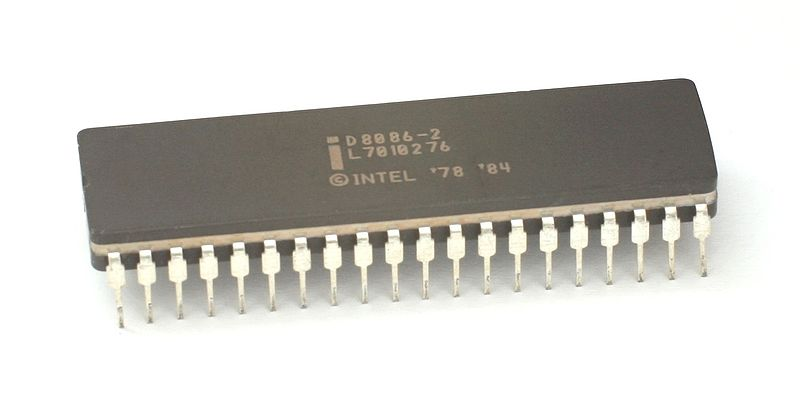
\includegraphics[width=0.3\textwidth]{../x8664-encoding/Intel8086}};
\end{tikzpicture}
\begin{itemize}
    \item 1979 Intel processor
    \item 4 general purpose 16-bit registers: AX, BX, CX, DX
    \item 4 special 16-bit registers: SI, DI, BP, SP
\end{itemize}
\end{frame}

\begin{frame}{8086 instruction encoding: simple}
\begin{itemize}
    \item special cases: 1-byte instructions:
    \begin{itemize}
    \item anything with no arguments
    \item push ax, push bx, push cx, \ldots (dedicated opcodes)
    \item pop ax, \ldots
    \end{itemize}
\end{itemize}
\end{frame}

\begin{frame}{8086 instruction encoding: two-arg}
\begin{itemize}
    \item 1-byte opcode
    \item sometimes {\tt ModRM} byte:
        \begin{itemize}
        \item 2-bit ``mod'' and 
        \item 3-bit register number (source or dest, depends on opcode) and
        \item 3-bit ``r/m'' (register or memory)
        \end{itemize}
    \item ``mod'' + ``r/m'' specify one of:
        \begin{itemize}
        \item {\tt \%reg} (mod = {\tt 11})
        \item {\tt (\%bx/\%bp, \%si/\%di)}
        \item {\tt (\%bx/\%si/\%di)}
        \item {\tt offset(\%bx/\%bp/,\%si/\%di)} (8- or 16-byte offset)
        \end{itemize}
    \item non-intuitive table
\end{itemize}
\end{frame}

\begin{frame}{16-bit ModRM table}
\begin{tikzpicture}
\node (table) {
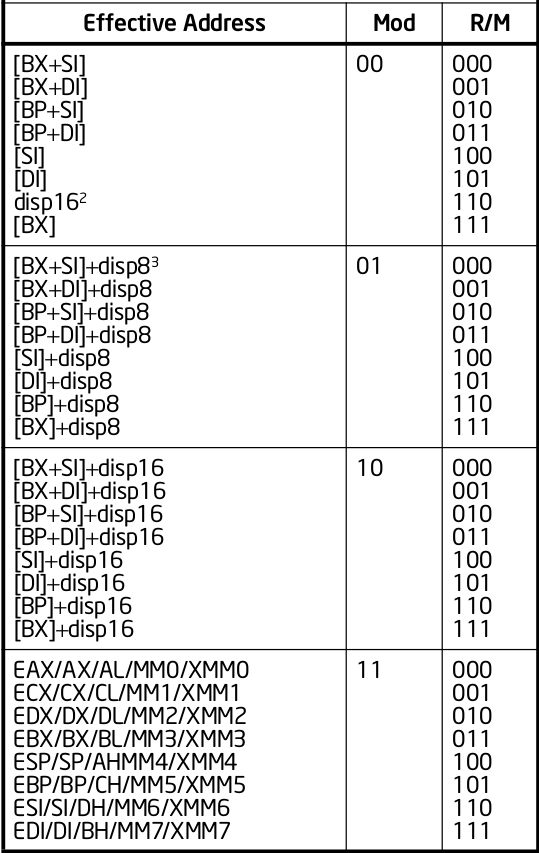
\includegraphics[height=0.8\textheight]{../x8664-encoding/16bitmodrm}
};
\begin{visibleenv}<2>
\node[anchor=north west,align=left] at (table.north east) {
    e.g. \texttt{add \%bl, \%cl} \\
    (Intel syntax: \texttt{add CL, BL}) \\
    Intel manual: \\
    \texttt{02 /r}: \texttt{ADD r8 {\normalfont(dest)}, r/m8} \\
    \texttt{/r} means ModRm byte with reg set to reg\# \\
    ~ \\
    opcode = \texttt{0x02}
    ModRM byte = \\
    \texttt{11} (mod) / \texttt{001} (reg: \%cl) / \texttt{011} (r/m: \%bl) \\
    or \texttt{1100 1011}
    ~ \\
    final encoding: \texttt{02 cb}
};
\end{visibleenv}
\end{tikzpicture}
\end{frame}

\begin{frame}{8086 evolution}
\begin{itemize}
\item Intel 8086 --- 1979, 16-bit registers
\item Intel (80)386 --- 1986, 32-bit registers
\item AMD K8 --- 2003, 64-bit registers
\end{itemize}
\end{frame}

\begin{frame}{x86 modes}
\begin{itemize}
\item x86 has multiple \myemph{modes}
\item maintains compatiblity
\item e.g.: modern x86 processor can work like 8086
    \begin{itemize}
    \item called ``real mode''
    \end{itemize}
\item different mode for 32-bit/64-bit
\item same basic encoding; some sizes change
\end{itemize}
\end{frame}

\begin{frame}{32-bit ModRM table}
\begin{tikzpicture}
\node (table) {
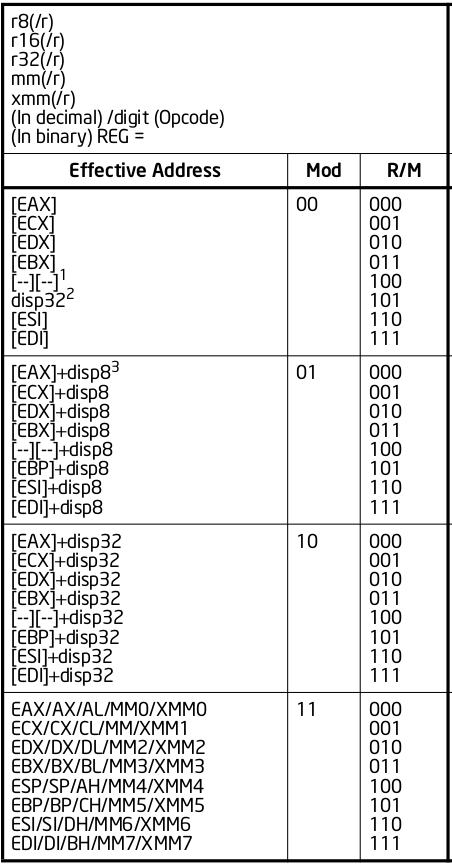
\includegraphics[height=0.8\textheight]{../x8664-encoding/32bitmodrm}
};
\begin{visibleenv}<2>
\node[anchor=north west,align=left] at (table.north east) {
    general pattern for 32-bit x86 register numbering: \\
    AX = 0, CX, DX, BX, SP, BP, SI, DI = 7 \\
    ~ \\
    not all registers treated equally to make space for \\
    special types of addressing: \\
    (base + index * scale, constant address)
};
\end{visibleenv}
\end{tikzpicture}
\end{frame}

\begin{frame}{32-bit addition: SIB bytes}
\begin{itemize}
\item 8086 addressing modes made registers different
\item 32-bit mode got rid of this (mostly)
\item problem: not enough spare bits in {\tt ModRM} byte
\item solution: if ``r/m'' bits = {\tt 100} (4, normally ESP), extra ``SIB'' byte:
    \begin{itemize}
    \item 2 bit \myemph<2>{scale}: {\tt 00} is 1, {\tt 01} is 2, {\tt 10} is 4, {\tt 11} is 8
    \item 3 bit \myemph<3>{index}: index register number
    \item 3 bit \myemph<4>{base}: base register number
    \end{itemize}
\item {\tt (\myemph<4>{\%baseReg},\myemph<3>{\%indexReg},\myemph<2>{scale})}
\end{itemize}
\end{frame}

\begin{frame}{intel manual: SIB table}
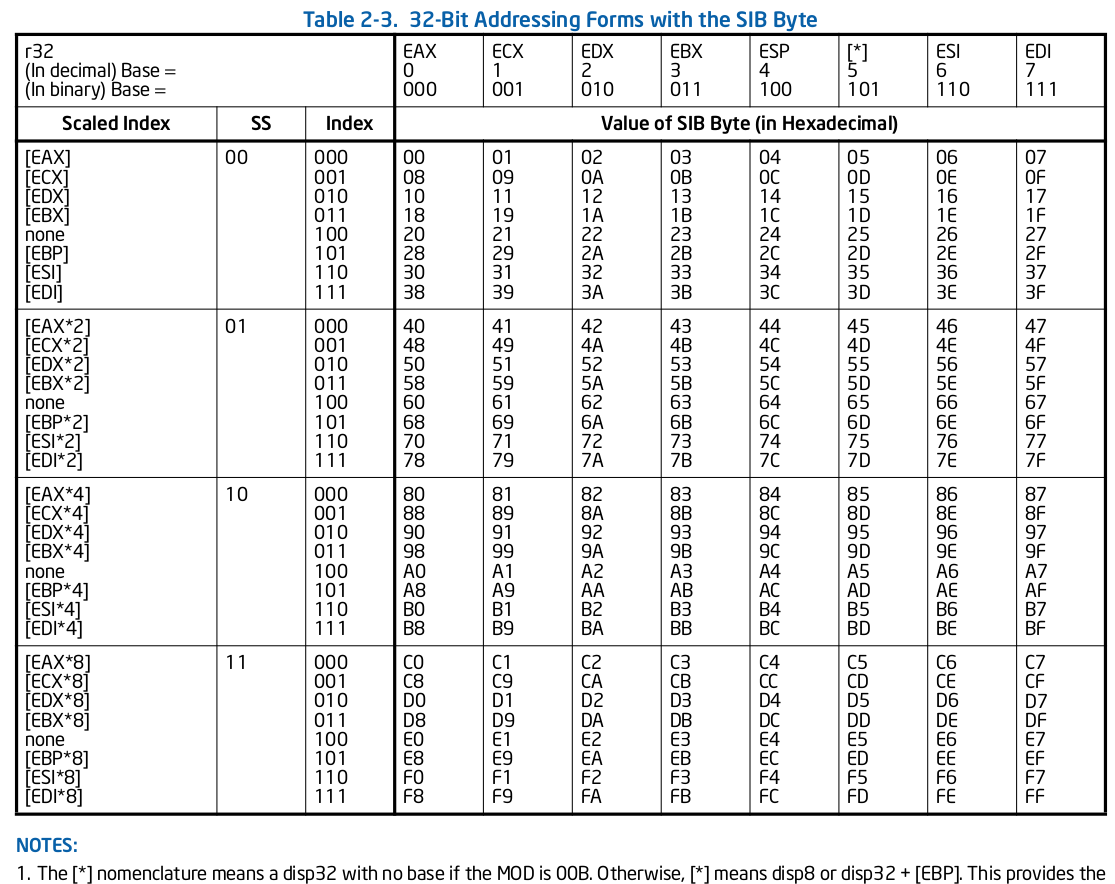
\includegraphics[height=0.9\textheight]{../x8664-encoding/32bitsib}
\end{frame}

\begin{frame}{basic 32-bit encoding}
\begin{tikzpicture}
\begin{scope}[start chain=going right,node distance=0mm,every node/.style={on chain,draw,font=\small,minimum height=1cm}]
\node { opcode }; \node[dashed] { Mod | Reg{\fontsize{9}{10}\selectfont/Opcode} | R/M }; \node[dashed] {SIB byte}; \node[dashed] {displacement}; \node[dashed] {immediate};
\end{scope}
\end{tikzpicture}
\begin{itemize}
\item dashed: not always present
\item opcodes: 1-3 bytes
    \begin{itemize}
    \item some 5-bit opcodes, with 3-bit register field
    \item (alternate view: 8-bit opcode with fixed register)
    \item sometimes Reg part of ModRM used as add'tl part of opcode
    \end{itemize}
\item displacement, immediate: 1, 2, or 4 bytes
    \begin{itemize}
    \item or, rarely, 8 bytes
    \end{itemize}
\end{itemize}
\end{frame}



\subsection{exercise}
\usetikzlibrary{chains}
\begin{frame}{exercise 1} 
\begin{tikzpicture}
\begin{scope}[start chain=going right,node distance=0mm,every node/.style={on chain,draw,font=\small,minimum height=1cm}]
\node (opcode) { opcode }; \node[dashed] { mod | reg{\fontsize{9}{10}\selectfont/opcode} | r/m}; \node[dashed] {scale / idx / base}; \node[dashed] {displacement}; \node[dashed] {immediate};
\end{scope}
\node[anchor=north west] (modrmtbl) at (opcode.south west) {
    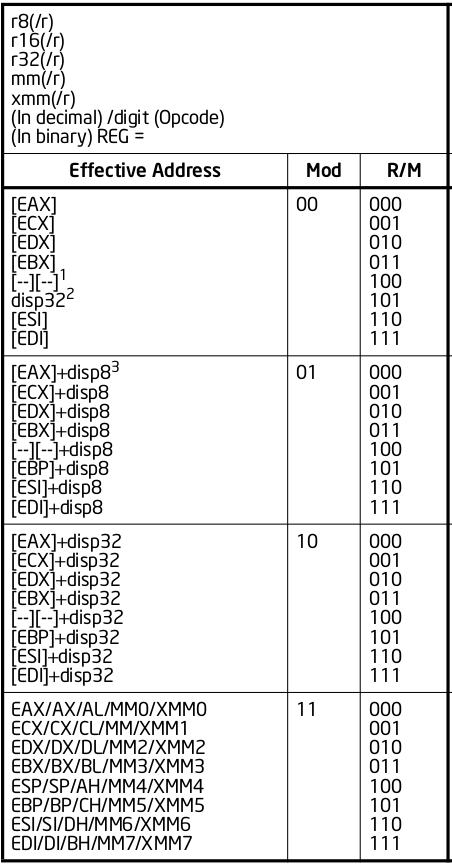
\includegraphics[height=0.8\paperheight]{../x8664-encoding/32bitmodrm}
};
\node[anchor=north west] (bts manual)at (modrmtbl.north east) {
    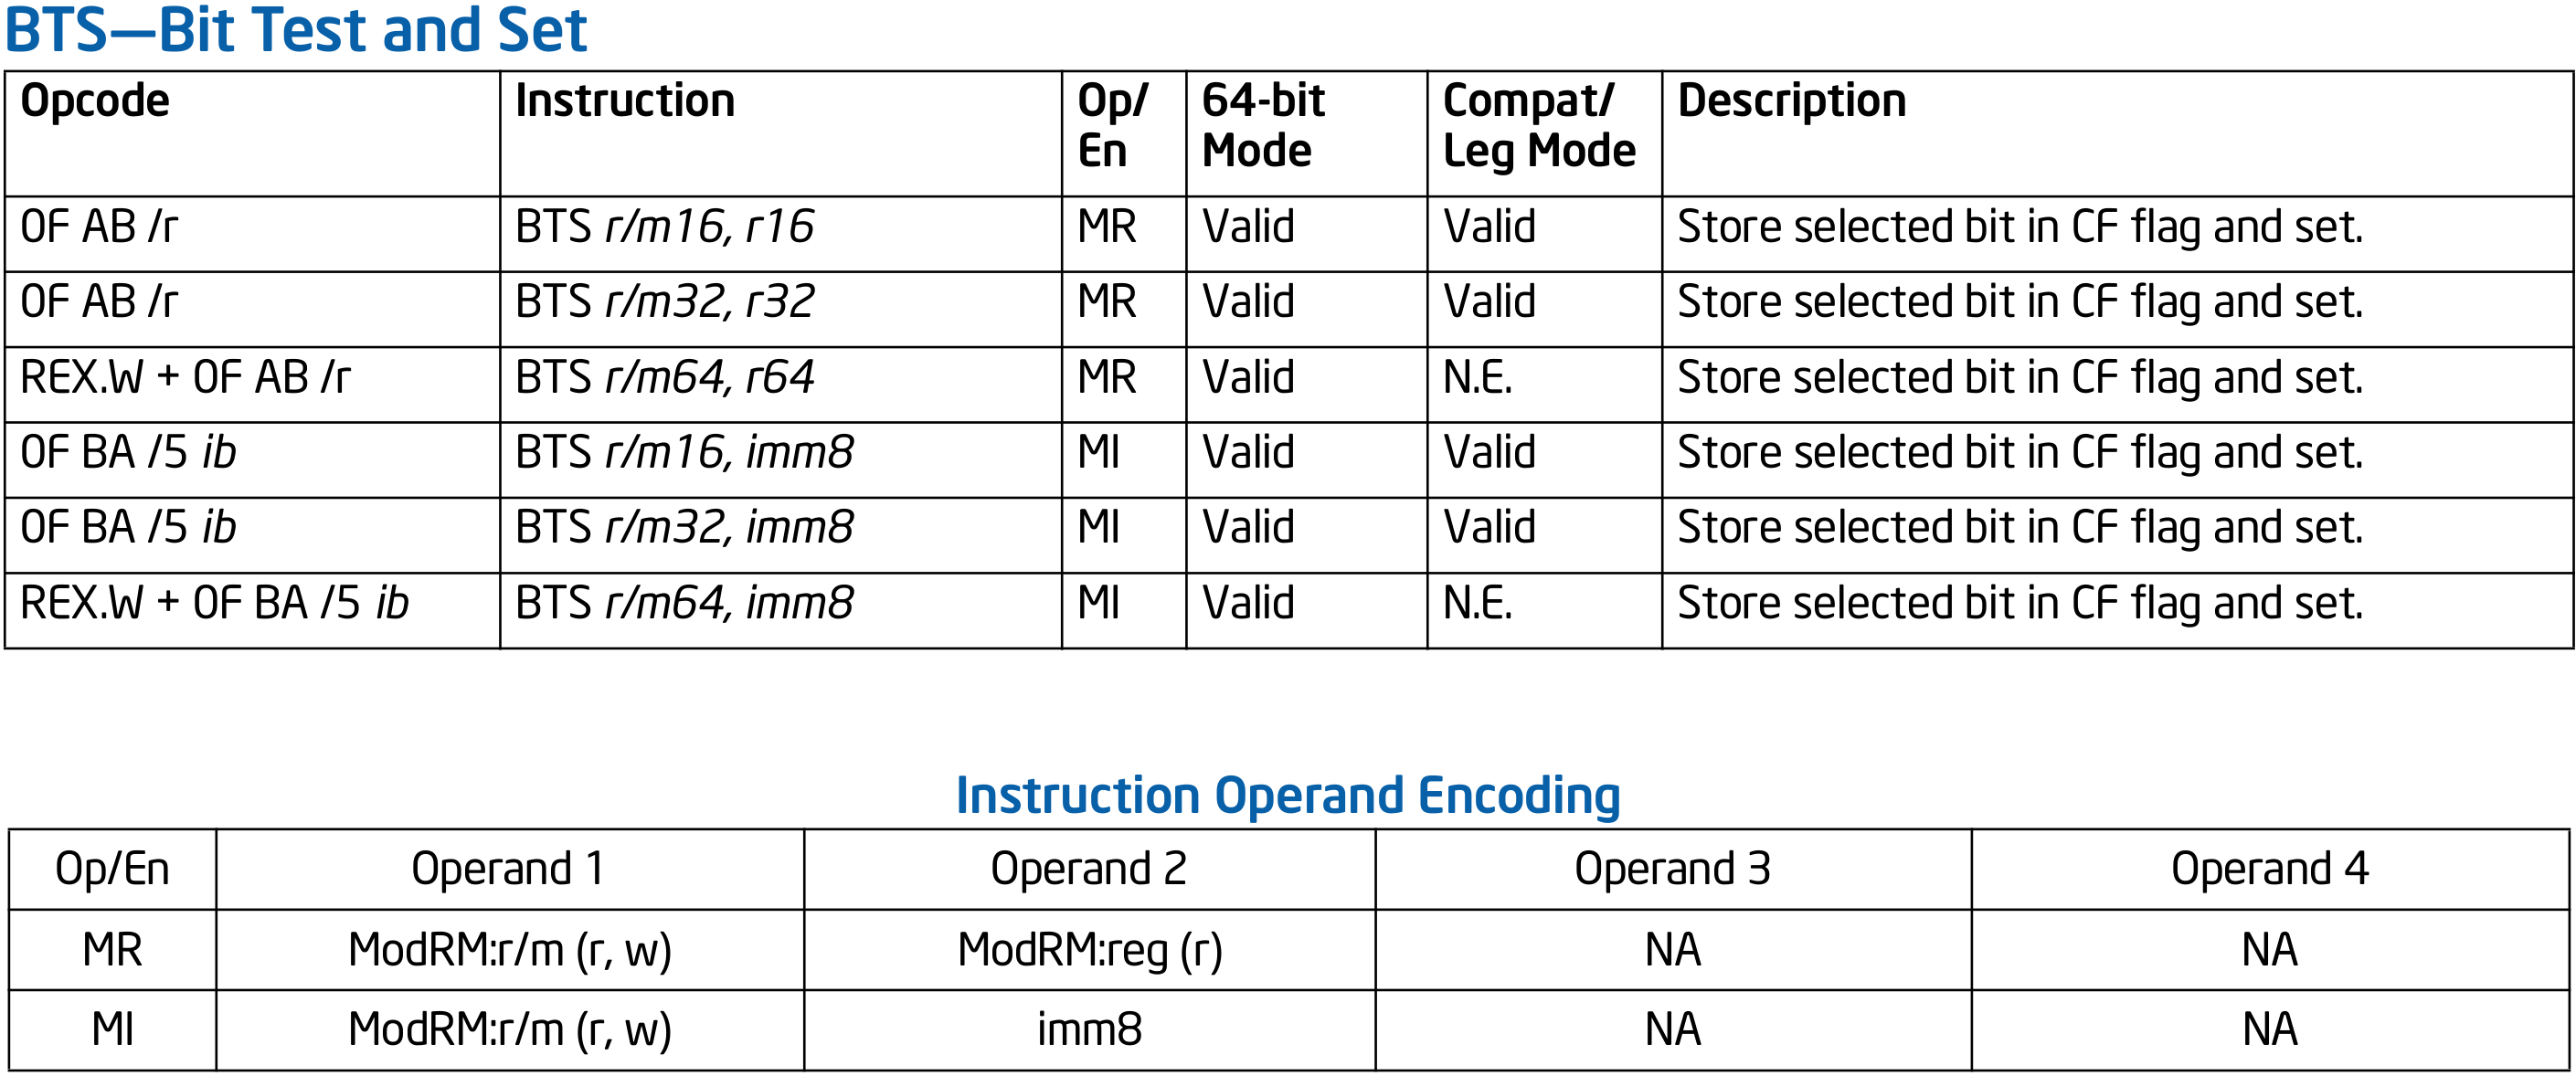
\includegraphics[width=0.75\textwidth]{../x8664-encoding/bts-manual}
};
\node[anchor=north west,align=left] (bts ex) at (bts manual.south west) {
    exercise: encode \texttt{btsl \$7, 4(\%rax)} \\
    (Intel syntax: \texttt{BTS DWORD PTR[RAX+4], 7})
};
\end{tikzpicture}
\end{frame}


\subsection{adding 64-bit}
\usetikzlibrary{arrows.meta,shapes.multipart}

\begin{frame}{what about 64-bit?}
\begin{itemize}
\item adds 8 more registers --- more bits for reg \#?
\item didn't change encoding for existing instructions, so\ldots
\item \myemph{instruction prefix} ``REX''
    \begin{itemize}
    \item 32-bit x86 already had many prefixes
    \end{itemize}
\item also selects 64-bit version of instruction
\end{itemize}
\end{frame}

\begin{frame}{REX prefix}
\begin{tikzpicture}
    \node[draw,rectangle split,rectangle split horizontal, rectangle split parts=5,
        label={north:REX prefix byte}] (rexbyte) {
        {\tt 0100}
        \nodepart{two}
        w
        \nodepart{three}
        r
        \nodepart{four}
        s
        \nodepart{five}
        b
    };
    \node[anchor=north west,align=left] (wExplain) at ([yshift=-5cm,xshift=.5cm]rexbyte.five south) {
        {\tt 1} if 64-bit values ({\tt \%rax}, etc. or from memory)\\
        {\tt 0} if 32-bit values ({\tt \%eax}, etc. or from memory)
    };
    \draw[thick,-Latex] (rexbyte.two south) |- (wExplain.west);
    \node[anchor=south west] (rExplain) at ([yshift=1mm]wExplain.north west) {
        extra bit for ModRM reg field
    };
    \draw[thick,-Latex] (rexbyte.three south) |- (rExplain.west);
    \node[anchor=south west] (sExplain) at ([yshift=1mm]rExplain.north west) {
        extra bit for SIB byte index reg field
    };
    \draw[thick,-Latex] (rexbyte.four south) |- (sExplain.west);
    \node[anchor=south west, align=left] (bExplain) at ([yshift=1mm]sExplain.north west) {
        extra bit for ModRM r/m \\ or SIB base reg field
    };
    \draw[thick,-Latex] (rexbyte.five south) |- (bExplain.west);
\end{tikzpicture}
%\vspace{.5cm}
%\item 4-bit constant 0100
%\item 1-bit ``w'': 1 if 64-bit operands
%\item 1-bit ``r'': extra bit for ModRM register number
%\item 1-bit ``s'': extra bit for SIB index register number
%\item 1-bit ``b'': extra bit for ``r/m'' or SIB index register number 
%    \begin{itemize}
%    \item or modify in-opcode register number
%    \end{itemize}
%\end{itemize}
\end{frame}



\subsection{exercise}
\begin{frame}{64-bit REX exercise (1)}
    \begin{itemize}
    \item \texttt{add \%eax, \%ecx} (Intel: {\tt ADD ecx, eax})
        \begin{itemize}
        \item {\tt 01} (opcode) {\tt c1} (MOD: 11 / REG: 000 (eax) / R\/M: 001 (ecx))
        \end{itemize}
    \item exercise 2a: \texttt{add \%eax, \%r10d} (Intel: {\tt ADD r9d, eax}) = ???
        \begin{itemize}
        \item REX prefix + {\tt 01} + MOD-REG-R/M byte
        \end{itemize}
    \vspace{.5cm}
    \item REX prefix:
        \begin{itemize}
        \item {\tt 0100}
        \item w (is 64-bit values?)
        \item r (extra bit for Reg field)
        \item s (extra bit for SIB index reg)
        \item b (extra bit for R/M or SIB base field)
        \end{itemize}
    \end{itemize}
\end{frame}

\begin{frame}{64-bit REX exercise (2)}
    \begin{itemize}
    \item \texttt{add \%eax, \%ecx} (Intel: {\tt ADD ecx, eax})
        \begin{itemize}
        \item {\tt 01} (opcode) {\tt c1} (MOD: 11 / REG: 000 (eax) / R\/M: 001 (ecx))
        \end{itemize}
    \item exercise 2b: \texttt{add \%rax, \%rcx} (Intel: {\tt ADD rcx, rax}) = ???
        \begin{itemize}
        \item REX prefix + {\tt 01} + MOD-REG-R/M byte
        \end{itemize}
    \vspace{.5cm}
    \item REX prefix:
        \begin{itemize}
        \item {\tt 0100}
        \item w (is 64-bit values?)
        \item r (extra bit for Reg field)
        \item s (extra bit for SIB index reg)
        \item b (extra bit for R/M or SIB base field)
        \end{itemize}
    \end{itemize}
\end{frame}


\subsection{encoding overall}
\begin{frame}{overall encoding}
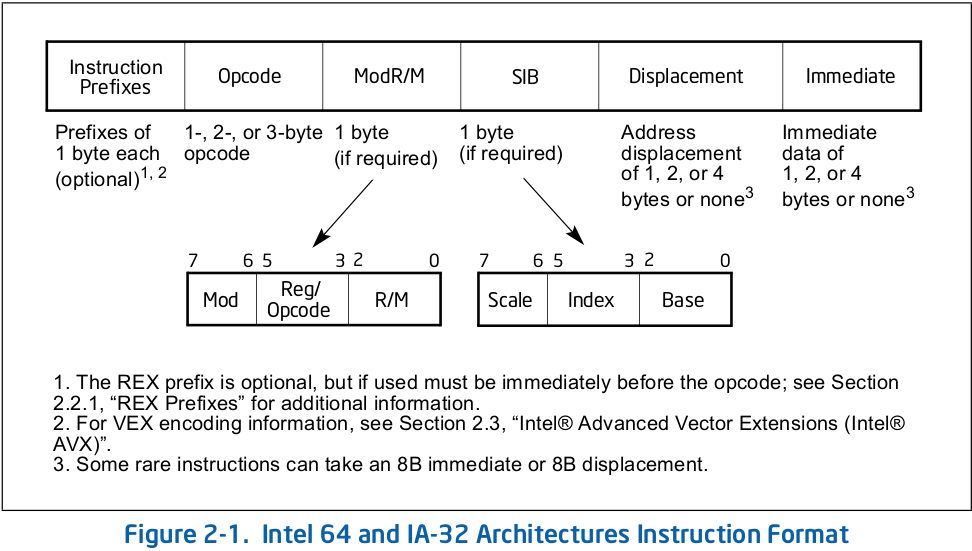
\includegraphics[width=\textwidth]{../x8664-encoding/IntelFig21}
\end{frame}


\subsection{misc prefixes}

\begin{frame}<1>[label=prefixes]{instruction prefixes}
    \begin{itemize}
    \item REX (64-bit and/or extra register bits)
    \item VEX (SSE/AVX instructions; other new instrs.)
    \item operand/address-size change (64/32 to 16 or vice-versa)
    \item {\tt LOCK} --- synchronization between processors
    \item \myemph<2>{{\tt REPNE/REPNZ/REP/REPE/REPZ} --- turns instruction into loop}
    \item segment overrides
    \end{itemize}
\end{frame}




\subsection{examples}

\begin{frame}[fragile,label=x86ex1]{x86 encoding example (1)}
    \begin{itemize}
    \item \lstinline|pushq %rax| encoded as {\tt 50}
        \begin{itemize}
        \item 5-bit opcode {\tt 01010} plus 3-bit register number {\tt 000} \\
        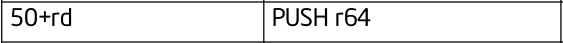
\includegraphics[width=0.4\textwidth]{../x8664-encoding/intel-manual-push-ex1}
        \end{itemize}
    \item \lstinline|pushq %r13| encoded as {\tt 41 55}
        \begin{itemize}
        \item {\tt 41}: REX prefix {\tt 0010} (constant), w:{\tt 0}, r:{\tt 0}, s:{\tt 0}, b:{\tt \color{blue!80!black}{1}}
        \item w = {\tt 0} because push is never 32-bit in 64-bit mode
        \item {\tt 55}: 5-bit opcode {\tt 01010}; 3-bit reg \# {\tt \color{green!80!black}{101}}
        \item 4-bit reg \# {\tt \color{blue!80!black}{1}\color{green!80!black}{101}} = 13
        \end{itemize}
    \end{itemize}
\end{frame}

\begin{frame}[fragile,label=x86ex2]{x86 encoding example (2)}
    \begin{itemize}
    \item \lstinline|addl 0x12345678(%rax,%rbx,2), %ecx|
    \item {\tt 03}: opcode --- add r/m32 into r32 
        \begin{itemize}
        \item
            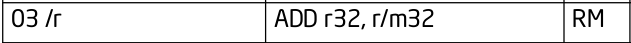
\includegraphics[width=0.4\textwidth]{../x8664-encoding/intel-manual-addl-ex1.png}
            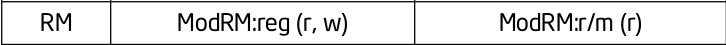
\includegraphics[width=0.4\textwidth]{../x8664-encoding/intel-manual-addl-ex2.png}
        \end{itemize}
    \item {\tt 8c}: ModRM: mod = {\tt 10}; reg = {\tt 001}, r/m: {\tt 100}
        \begin{itemize}
        \item reg = {\tt 001} = {\tt \%ecx} (table)
        \item SIB byte + 32-bit displacement (table)
        \end{itemize}
    \item {\tt 58}: SIB: scale = {\tt 01}, index = {\tt 011}, base = {\tt 000}
        \begin{itemize}
        \item index {\tt 011} = {\tt \%rbx}; base {\tt 000} = {\tt \%rax};
        \end{itemize}
    \item {\tt 78 56 32 12}: 32-bit constant {\tt 0x12345678}
    \end{itemize}
\end{frame}

\begin{frame}[fragile,label=x86ex3]{x86 encoding example (3)}
    \begin{itemize}
    \item \lstinline|addq 0x12345678(%r10,%r11,2), %rax|
    \item {\tt 4b}: REX prefix {\tt 0100}+w:{\tt \myemph<2>{1}}, r:{\tt \textcolor{violet!80!black}{\myemph<3>{0}}}, s:{\tt \textcolor{blue!80!black}{\myemph<4>{1}}}, b:{\tt \textcolor{green!80!black}{\myemph<5>{1}}}
    \item {\tt 03}: opcode --- add r/m64 to r64 (with \myemph<2>{REX.w})
    \item {\tt 84}: ModRM: mod = {\tt 10}; reg = {\tt 000}, r/m: {\tt 100}
        \begin{itemize}
        \item reg = {\tt \textcolor{violet!80!black}{\myemph<3>{0}}000} = \%rax
        \item SIB byte + 32-bit displacement (table)
        \end{itemize}
    \item {\tt 5a}: SIB: scale = {\tt 01}, index = {\tt 011}, base = {\tt 010}
        \begin{itemize}
        \item with REX: index = {\tt \textcolor{blue!80!black}{\myemph<4>{1}}011} (11), base = {\tt \textcolor{green!80!black}{\myemph<5>{1}}010} (10)
        \end{itemize}
    \item {\tt 78 56 32 12}: 32-bit constant {\tt 0x12345678}
    \end{itemize}
\end{frame}

\begin{frame}[fragile,label=x86ex4]{x86 encoding example (4)}
    \begin{itemize}
    \item \lstinline|movq %fs:0x10,%r13|
    \item {\tt 64}: FS segment override
    \item {\tt 48}: REX: {\tt w}: 1 (64-bit), {\tt r}: \textcolor{violet!80!black}{\tt \myemph<2>{1}}, {\tt s}: \textcolor{blue!80!black}{\tt \myemph<3>{0}}, {\tt b}: \textcolor{green!80!black}{\tt \myemph<4>{0}}
    \item {\tt 8b}: opcode for MOV memory to register
    \item {\tt 2c}: ModRM: mod = {\tt 00}, reg = {\tt 101}, r/m: {\tt 100}
        \begin{itemize}
        \item with REX: reg = {\tt \textbf{\textcolor{violet!80!black}{\myemph<2>{1}}}101} [\%r12]; r/m = {100} (SIB follows)
        \end{itemize}
    \item {\tt 25}: SIB: scale = {\tt 00}; index = {\tt (\textcolor{blue!80!black}{\myemph<3>{0}})100}; base = {\tt (\textcolor{green!80!black}{\myemph<4>{0}})101}
        \begin{itemize}
        \item no register/no register in table
        \end{itemize}
    \item {\tt 10 00 00 00}: 4-byte constant {\tt 0x10}
    \end{itemize}
\end{frame}




\subsection{some impossible instructions}

\begin{frame}[fragile,label=x8664impos]{x86-64 impossibilities}
\lstset{
    language=myasm,
    style=small,
    moredelim={**[is][\sout<all:1>]{~sout~}{~endsout~}},
}
    \begin{itemize}
    \item \myemph{illegal}: \lstinline|~sout~movq 0x12345678ab(%rax), %rax~endsout~|
        \begin{itemize}
        \item maximum 32-bit displacement
        \item \lstinline|movq 0x12345678ab, %rax| okay
            \begin{itemize}
            \item extra {\tt mov} opcode for {\tt \%rax} only
            \end{itemize}
        \end{itemize}
    \item \myemph{illegal}: \lstinline|~sout~movq $0x12345678ab, %rbx~endsout~|
        \begin{itemize}
        \item maximum 32-bit constant
        \item \lstinline|movq $0x12345678ab, %rax| okay
        \end{itemize}
    \item \myemph{illegal}: \lstinline|~sout~pushl %eax~endsout~|
        \begin{itemize}
        \item no 32-bit push/pop in 64-bit mode
        \item but 16-bit allowed (operand size prefix byte {\tt 66})
        \end{itemize}
    \item \myemph{illegal}: \lstinline|~sout~movq (%rax, %rsp), %rax~endsout~|
        \begin{itemize}
        \item cannot use \lstinline|%rsp| as index register
        \item \lstinline|movq (%rsp, %rax), %rax| okay
        \end{itemize}
    \end{itemize}
\end{frame}



\subsection{position-independence} 
\begin{frame}[fragile,label=picVNot]{position dependence}
\begin{itemize}
\item two ways of encoding addresses in x86-64 assembly:
    \begin{itemize}
    \item address in little endian (typically 32-bits --- limit on executable size)
    \item difference between address and \%rip (next instruction address)
    \end{itemize}
\end{itemize}
\hrule
{\tt
\begin{tabular}{l|l}
movb label, \%al & 8a 04 25 {\normalfont\it label's addr (32 bit)} \\
jmp *label & ff 24 25 {\normalfont\it label's addr (32 bit)} \\
movb label(\%rip), \%al & 8a 05 {\normalfont\it \%rip - label's addr (32 bit)} \\
jmp label & e9 {\normalfont\it \%rip - label's addr (32 bit)} \\
\end{tabular}
}
how to know which? --- check manual
\end{frame}


\subsection{PIC: which should be exercise?}
\begin{frame}{position-independence: which to use?}
\begin{itemize}
\item suppose we're inserting ``evil'' code \\
at changing addresses in executable's memory
\item which of the following do we want absolute encoding for? \\
(i.e. which would absolute encoding be easier than relative)
    \begin{itemize}
    \item A. address of a jump from evil code to function at fixed loc in executable
    \item B. address of a jump in a loop in the ``evil'' code
    \item C. address of a string in the ``evil'' code
    \item D. address of a string in the executable
    \end{itemize}
\end{itemize}
\end{frame}




\section{running example}
\begin{frame}[fragile]{running example}
\begin{Verbatim}[fontsize=\small]
$ file mystery
mystery: ELF 64-bit LSB pie executable, x86-64,
version 1 (SYSV), dynamically linked,
interpreter /lib64/ld-linux-x86-64.so.2,
BuildID[sha1]=9819a3cfb39d01ad2a376c54318f104139422a8f,
for GNU/Linux 3.2.0, stripped
\end{Verbatim}
\begin{itemize}
\item LSB = little endian
\item pie = position-independent executable
\item interpreter = program that loads this
\end{itemize}
\end{frame}

\begin{frame}[fragile]{aside: file(1)}
\begin{Verbatim}[fontsize=\small]
$ man file
FILE(1)                      General Commands Manual                    FILE(1)

NAME
       file — determine file type

....
\end{Verbatim}
\hrule
\begin{itemize}
\item looks for ``magic numbers'' near beginning of file data
\item hand-managed database of common patterns
\end{itemize}
\end{frame}

\begin{frame}[fragile]{from file's source}
\begin{Verbatim}[fontsize=\scriptsize]
0   name        elf-le
>16 leshort     0       no file type,
!:mime  application/octet-stream
>16 leshort     1       relocatable,
!:mime  application/x-object
>16 leshort     2       executable,
!:mime  application/x-executable
>16 leshort     3       ${x?pie executable:shared object},

...
0   string      \177ELF     ELF
!:strength *2
>4  byte        0       invalid class
>4  byte        1       32-bit
>4  byte        2       64-bit
>5  byte        0       invalid byte order
>5  byte        1       LSB
>>0 use     elf-le
>5  byte        2       MSB
>>0 use     \^elf-le
>7  byte        0       (SYSV)
\end{Verbatim}
\end{frame}


\section{finding strings}

\begin{frame}[fragile]{finding strings}
\begin{Verbatim}[commandchars=~\{\},fontsize=\fontsize{9}{10}]
$ hexdump -c mystery
00000000  7f 45 4c 46 02 01 01 00  00 00 00 00 00 00 00 00  |.ELF............|
00000010  03 00 3e 00 01 00 00 00  c0 60 00 00 00 00 00 00  |..>......`......|
00000020  40 00 00 00 00 00 00 00  08 5e 03 00 00 00 00 00  |@........^......|
00000030  00 00 00 00 40 00 38 00  0d 00 40 00 1e 00 1d 00  |....@.8...@.....|
~textit{[... many more lines ...]}
00000e60  00 5f 49 54 4d 5f 64 65  72 65 67 69 73 74 65 72  |._ITM_deregister|
00000e70  54 4d 43 6c 6f 6e 65 54  61 62 6c 65 00 5f 5f 67  |TMCloneTable.__g|
00000e80  6d 6f 6e 5f 73 74 61 72  74 5f 5f 00 5f 49 54 4d  |mon_start__._ITM|
00000e90  5f 72 65 67 69 73 74 65  72 54 4d 43 6c 6f 6e 65  |_registerTMClone|
00000ea0  54 61 62 6c 65 00 77 61  64 64 63 68 00 63 6c 65  |Table.waddch.cle|
00000eb0  61 72 6f 6b 00 6e 6f 65  63 68 6f 00 6d 76 70 72  |arok.noecho.mvpr|
~textit{[... many more lines ...]}
\end{Verbatim}
\end{frame}

\begin{frame}{exercise: heuristic?}
    \begin{itemize}
    \item could scan through pages of hexdump for something interesting\ldots
    \vspace{.5cm}
    \item good heuristic for automating this process?
    \end{itemize}
\end{frame}

\begin{frame}[fragile]{strings utility (1)}
\begin{Verbatim}[fontsize=\fontsize{9}{10}]
$ strings mystery
/lib64/ld-linux-x86-64.so.2
*7lT1
A9B*
m8m7
_ITM_deregisterTMCloneTable
__gmon_start__
_ITM_registerTMCloneTable
waddch
clearok
\end{Verbatim}
\vspace{-1em}
\ldots
\begin{Verbatim}[fontsize=\fontsize{9}{10}]
        prints help
        identify object
        left
        down
        right
\end{Verbatim}
\vspace{-1em}
\ldots
\begin{Verbatim}[fontsize=\fontsize{9}{10}]
        save game
        quit
\end{Verbatim}
\end{frame}

\begin{frame}[fragile]{strings utility (2)}
\begin{Verbatim}[fontsize=\fontsize{9}{10}]
$ strings --bytes=40 mystery
character you want help for (* for all):
you feel a wrenching sensation in your gut
your armor appears to be weaker now. Oh my!
you feel a sting in your arm and now feel weaker
Level: %d  Gold: %-5d  Hp: %*d(%*d)  Str: %2d(%d)  Ac: %-2d  Exp: %d/%ld  %s
Ok, if you want to exit that badly, I'll have to allow it
Hello %s, just a moment while I dig the dungeon...
orry, but your terminal window has too few columns.
Sorry, but your terminal window has too few lines.
please specifiy a letter between 'A' and 'Z'
\end{Verbatim}
\ldots
\end{frame}

\begin{frame}{in Ghidra}
\small (after making new project, loading mystery file) \\
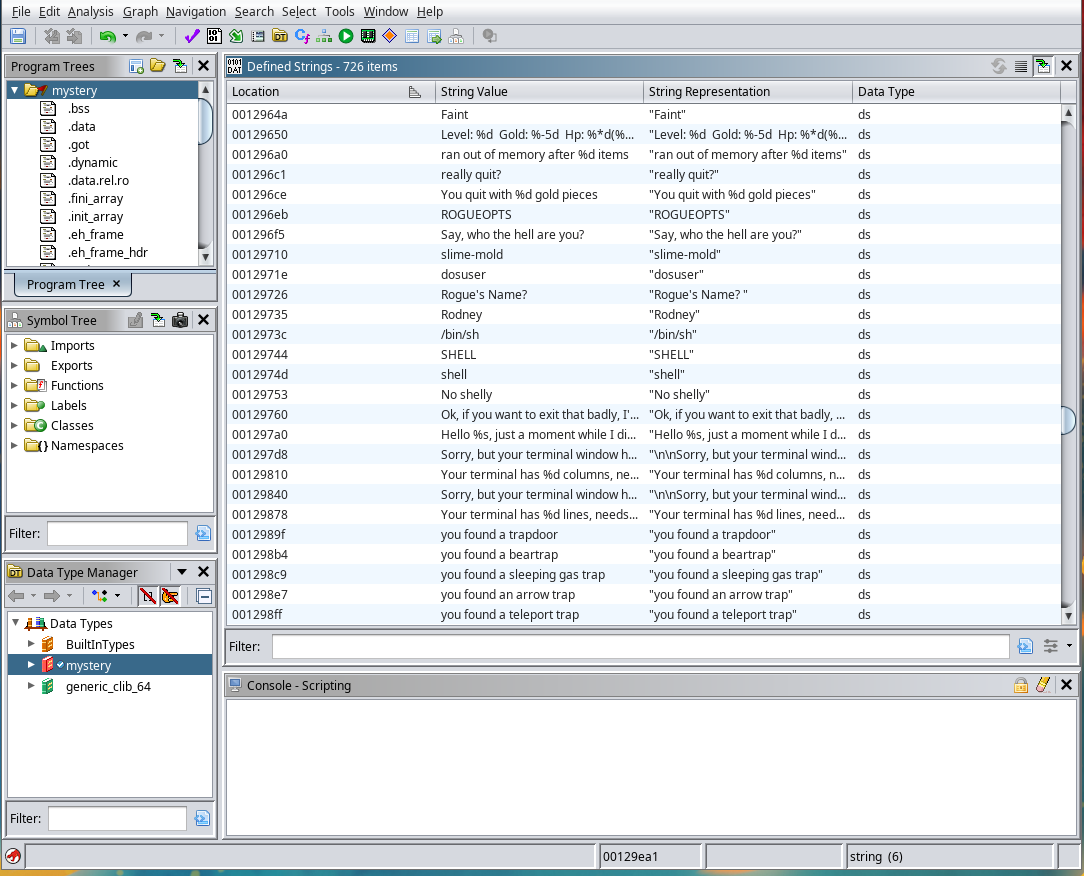
\includegraphics[width=0.8\textwidth]{../re-tools/ghidra-strings-mystery-ex}
\end{frame}



\section{finding library/system calls}

    % FIXME: objdump -R
    % FIXME: objdump -t

\begin{frame}[fragile]{libraries}
\begin{Verbatim}[fontsize=\small]
$ objdump --all-headers mystery
\end{Verbatim}
\ldots
\begin{Verbatim}[fontsize=\small]
Dynamic Section:
  NEEDED               libncurses.so.6
  NEEDED               libtinfo.so.6
  NEEDED               libc.so.6
\end{Verbatim}
\ldots
\end{frame}

\begin{frame}[fragile]{ncurses?}
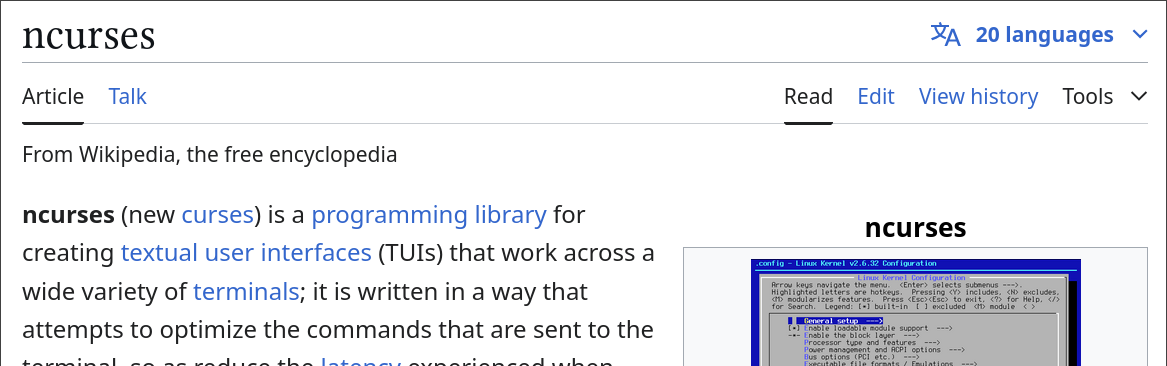
\includegraphics[width=\textwidth]{../re-tools/ncurses-wiki}
\end{frame}

\begin{frame}[fragile]{tinfo? (1)}
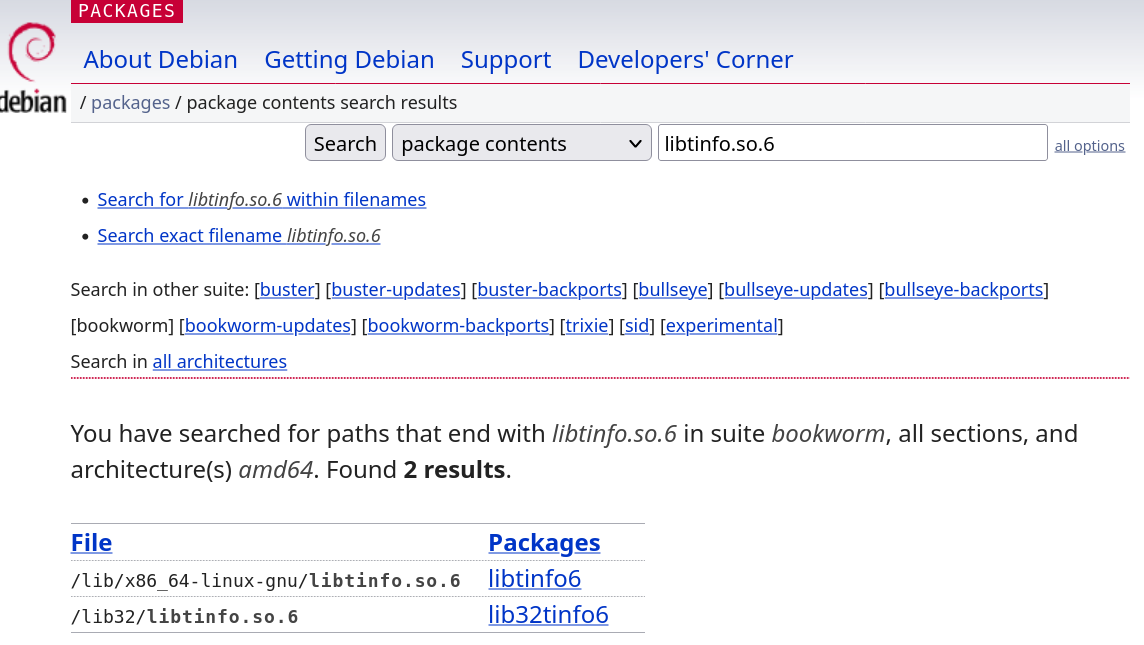
\includegraphics[width=0.7\textwidth]{../re-tools/deb-tinfo1}
\end{frame}

\begin{frame}[fragile]{tinfo? (2)}
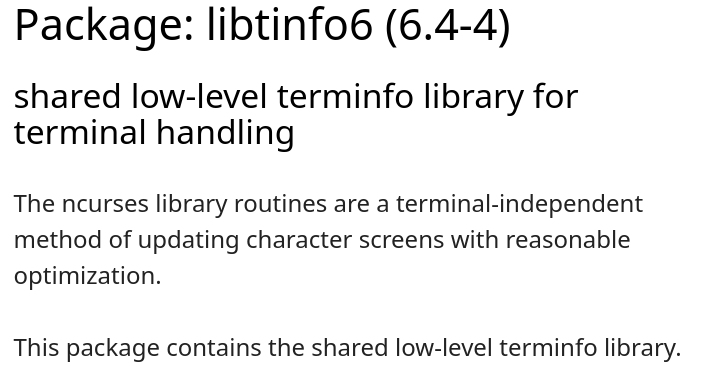
\includegraphics[width=0.7\textwidth]{../re-tools/deb-tinfo2}
\end{frame}

\begin{frame}[fragile]{library calls}
\begin{Verbatim}[fontsize=\fontsize{8}{9}]
$ objdump --dynamic-syms mystery

mystery:     file format elf64-x86-64

DYNAMIC SYMBOL TABLE:
0000000000000000      DF *UND*  0000000000000000 (GLIBC_2.3)  __ctype_toupper_loc
0000000000000000      DF *UND*  0000000000000000 (GLIBC_2.2.5) getenv
0000000000000000      DF *UND*  0000000000000000 (NCURSES6_5.0.19991023) wattrset
0000000000000000      DF *UND*  0000000000000000 (GLIBC_2.2.5) free
0000000000000000      DF *UND*  0000000000000000 (NCURSES6_TINFO_5.0.19991023) flushinp
0000000000000000      DF *UND*  0000000000000000 (GLIBC_2.2.5) localtime
0000000000000000      DF *UND*  0000000000000000 (GLIBC_2.34) __libc_start_main
\end{Verbatim}
\ldots
\begin{Verbatim}[fontsize=\fontsize{9}{10}]
0000000000000000      DF *UND*  0000000000000000 (GLIBC_2.2.5) setuid
\end{Verbatim}
\ldots
\end{frame}

\begin{frame}[fragile]{library calls (Ghidra)}
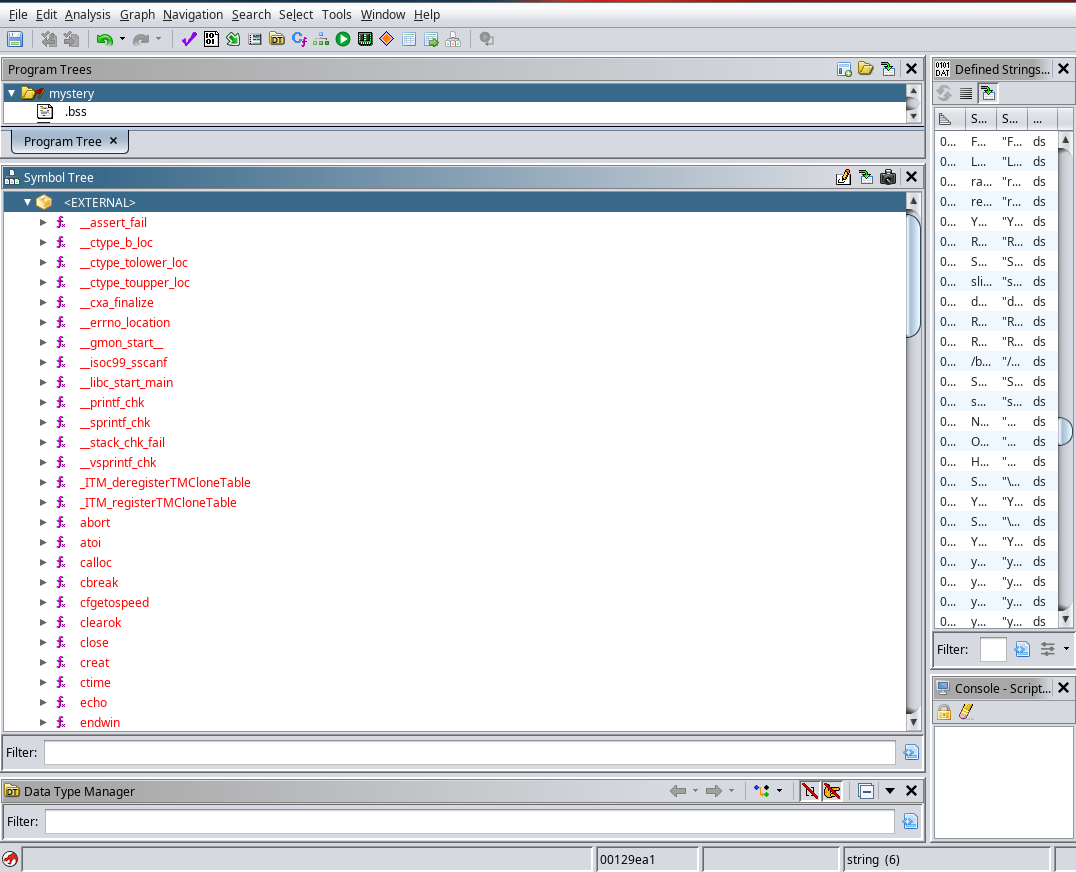
\includegraphics[width=\textwidth]{../re-tools/ghidra-mystery-ext}
\end{frame}

\begin{frame}[fragile]{finding library call uses}
{\small {\tt objdump --disassemble --dyanmic-reloc:}}
\begin{Verbatim}[fontsize=\fontsize{9}{10}]
0000000000005b00 <setuid@plt>:
    5b00:▶      f3 0f 1e fa          ▶  endbr64␣
    5b04:▶      f2 ff 25 fd d3 02 00 ▶  bnd jmp *0x2d3fd(%rip) 
			# 32f08 <setuid@GLIBC_2.2.5>
    5b0b:▶      0f 1f 44 00 00       ▶  nopl   0x0(%rax,%rax,1)
\end{Verbatim}
\ldots
\begin{Verbatim}[fontsize=\fontsize{9}{10}]
   2764f:▶      e8 ec e3 fd ff       ▶  call   5a40 <open@plt>
   27654:▶      89 05 fe 48 01 00    ▶  mov    %eax,0x148fe(%rip)        # 3bf58 <LINES@NCURSES6_TINFO_5.0.19991023+0x5244>
   2765a:▶      31 c0                ▶  xor    %eax,%eax
   2765c:▶      e8 2f e1 fd ff       ▶  call   5790 <getuid@plt>
   27661:▶      89 c7                ▶  mov    %eax,%edi
   27663:▶      31 c0                ▶  xor    %eax,%eax
   27665:▶      e8 96 e4 fd ff       ▶  call   5b00 <setuid@plt>
   2766a:▶      31 c0                ▶  xor    %eax,%eax
   2766c:▶      e8 cf e2 fd ff       ▶  call   5940 <getgid@plt>
   27671:▶      48 83 c4 08          ▶  add    $0x8,%rsp
\end{Verbatim}
\end{frame}

% FIXME: library call uses Ghidra


\section{disassembly, need for xrefs}
\begin{frame}[fragile]{disassembly issues (1)}
\begin{lstlisting}[language=myasm,style=size8]
.global main
main:
    call print_hello
    xorl %eax, %eax
    ret
.Lstr:
    .asciz "Hello!"
print_hello:
    leaq .Lstr(%rip), %rdi  // RDI <- .Lstr address
    jmp puts
\end{lstlisting}
\hrule
\begin{Verbatim}[fontsize=\fontsize{8}{9},commandchars=\\\{\}]
0000000000001139 <main>:
    1139:	e8 0a 00 00 00       	call   1148 <print_hello>
    113e:	31 c0                	xor    %eax,%eax
    1140:	c3                   	ret    
    \myemph{1141:	48                   	rex.W}
    \myemph{1142:	65 6c                	gs insb (%dx),%es:(%rdi)}
    \myemph{1144:	6c                   	insb   (%dx),%es:(%rdi)}
    \myemph{1145:	6f                   	outsl  %ds:(%rsi),(%dx)}
    \myemph{1146:	2e                   	cs}
\myemph{	...}
0000000000001148 <print_hello>:
    1148:	48 8d 3d f2 ff ff ff 	lea    -0xe(%rip),%rdi        # 1141 <main+0x8>
    114f:	e9 dc fe ff ff       	jmp    1030 <puts@plt>
\end{Verbatim}
\end{frame}

\begin{frame}[fragile]{disassembly issues}
\begin{Verbatim}[fontsize=\fontsize{8}{9},commandchars=\\\{\}]
0000000000001139 <main>:
    1139:	e8 0a 00 00 00       	call   1148 <print_hello>
    113e:	31 c0                	xor    %eax,%eax
    1140:	c3                   	ret    
    \myemph{1141:	48                   	rex.W}
    \myemph{1142:	65 6c                	gs insb (%dx),%es:(%rdi)}
    \myemph{1144:	6c                   	insb   (%dx),%es:(%rdi)}
    \myemph{1145:	6f                   	outsl  %ds:(%rsi),(%dx)}
    \myemph{1146:	2e                   	cs}
    \myemph{	...}
0000000000001148 <print_hello>:
    1148:	48 8d 3d f2 ff ff ff 	lea    -0xe(%rip),%rdi        # 1141 <main+0x8>
    114f:	e9 dc fe ff ff       	jmp    1030 <puts@plt>
\end{Verbatim}
\hrule
\begin{Verbatim}[fontsize=\fontsize{8}{9},commandchars=\\\{\}]
    1139:	e8 0a 00 00 00       	call   1148 <__cxa_finalize@plt+0x108>
    113e:	31 c0                	xor    %eax,%eax
    1140:	c3                   	ret    
    \myemph{1141:	48                   	rex.W}
    \myemph{1142:	65 6c                	gs insb (%dx),%es:(%rdi)}
    \myemph{1144:	6c                   	insb   (%dx),%es:(%rdi)}
    \myemph{1145:	6f                   	outsl  %ds:(%rsi),(%dx)}
    1146:	\myemph{2e 00} 48 8d          	cs add %cl,-0x73(%rax)
    114a:	3d f2 ff ff ff       	cmp    $0xfffffff2,%eax
    114f:	e9 dc fe ff ff       	jmp    1030 <puts@plt>
\end{Verbatim}
\end{frame}

\begin{frame}{finding assembly heuristics}
    \begin{itemize}
    \item objdump strategy, apparently:
        \begin{itemize}
        \item disassemble instructions starting at each symbol
        \item skip over strings of zero-bytes just before symbol
        \end{itemize}
    \item problem: can misidentify jumped to instructions
        \begin{itemize}
        \item especially if symbols stripped to save space/hinder reverse engineering
        \end{itemize}
    \item exercise: algorithm to fix?
        \begin{itemize}
        \item (Ghidra does this)
        \end{itemize}
    \end{itemize}
\end{frame}

% FIXME: exercise: Q: what to do about range of addresses given context?


\begin{frame}
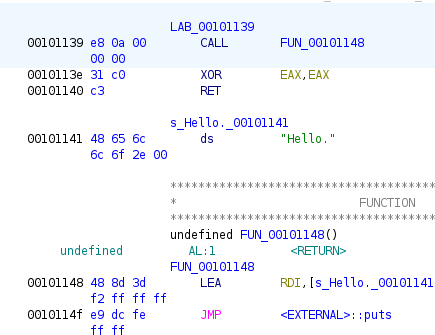
\includegraphics[width=\textwidth]{ghidra-disass-mixed-detail}
\end{frame}


\section{cross-references}
\begin{frame}{cross-references (1)}
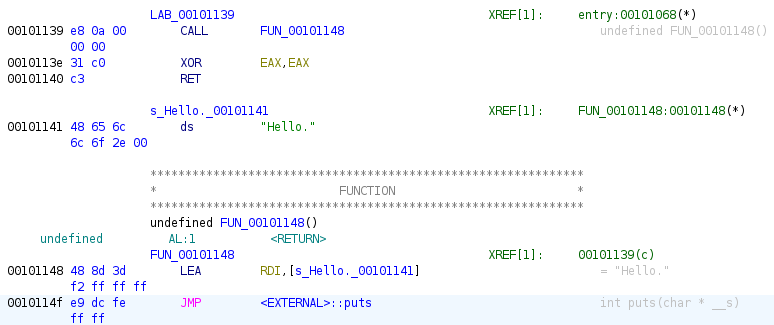
\includegraphics[width=\textwidth]{../re-tools/ghidra-disass-mixed-w-xref}
\end{frame}

\begin{frame}{cross-references idea}
    \begin{itemize}
    \item cross-reference idea:
    \item really useful to know where something is used
    \vspace{.5cm}
    \item do-able `by hand' with objdump and friends, but\ldots
        \begin{itemize}
        \item lots of bookkeeping, searching in text files, etc.
        \end{itemize}
    \end{itemize}
\end{frame}

\begin{frame}{more cross-references}
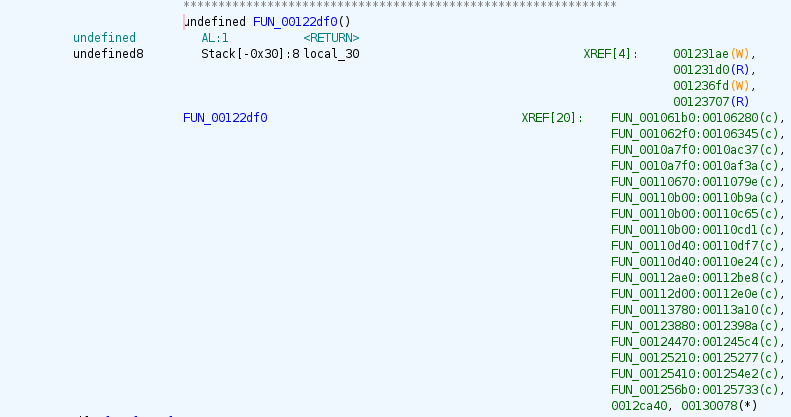
\includegraphics[width=\textwidth]{../re-tools/ghidra-mystery-xref-many}
\end{frame}




\section{high-level overviews}

\subsection{function callers/callees}
\begin{frame}{function callers?}
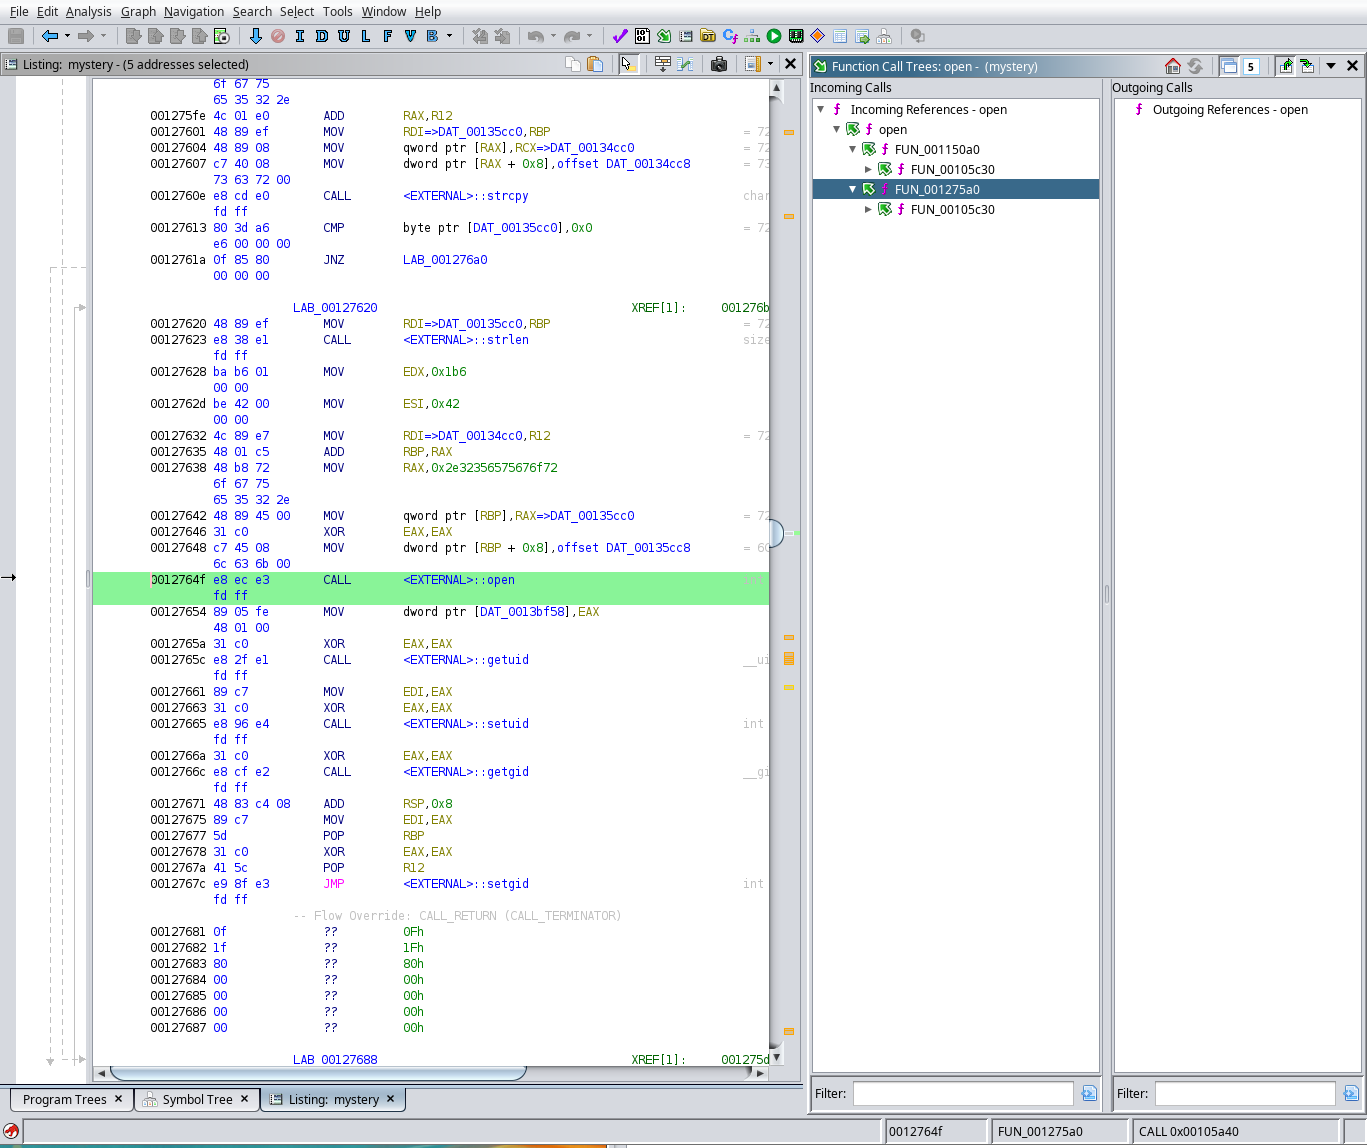
\includegraphics[width=\textwidth]{../re-tools/ghidra-symb-refs-ex}
\end{frame}

\begin{frame}{FUN\_12345678}
    \begin{itemize}
    \item Ghidra names functions without symbols based on address
    \item we can adjust that\ldots
    \end{itemize}
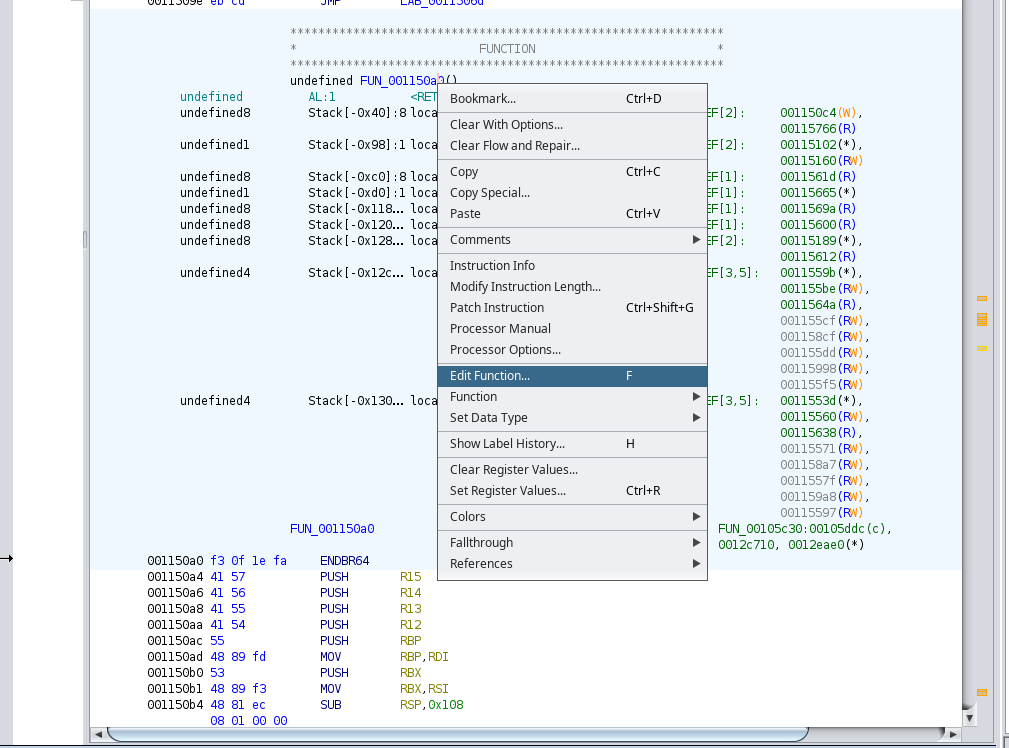
\includegraphics[width=0.45\textwidth]{../re-tools/ghidra-edit-func-cut}
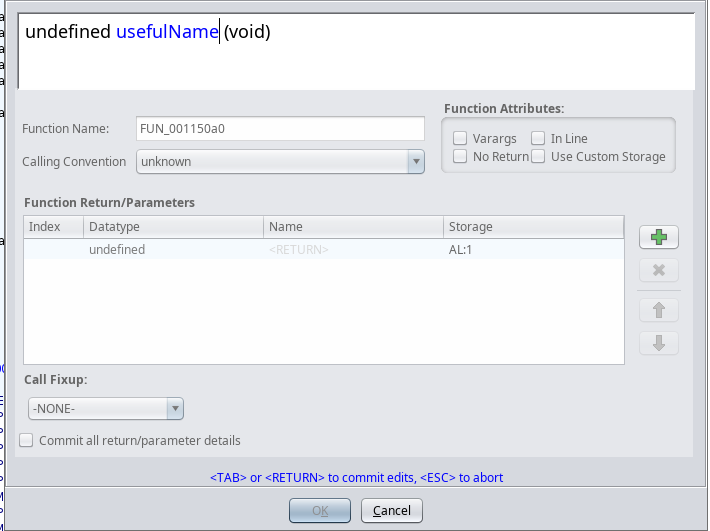
\includegraphics[width=0.45\textwidth]{../re-tools/ghidra-edit-func-dialog}
\end{frame}

 % FIXME: cleanup exercise

\subsection{control flow graphs}
\begin{frame}{}
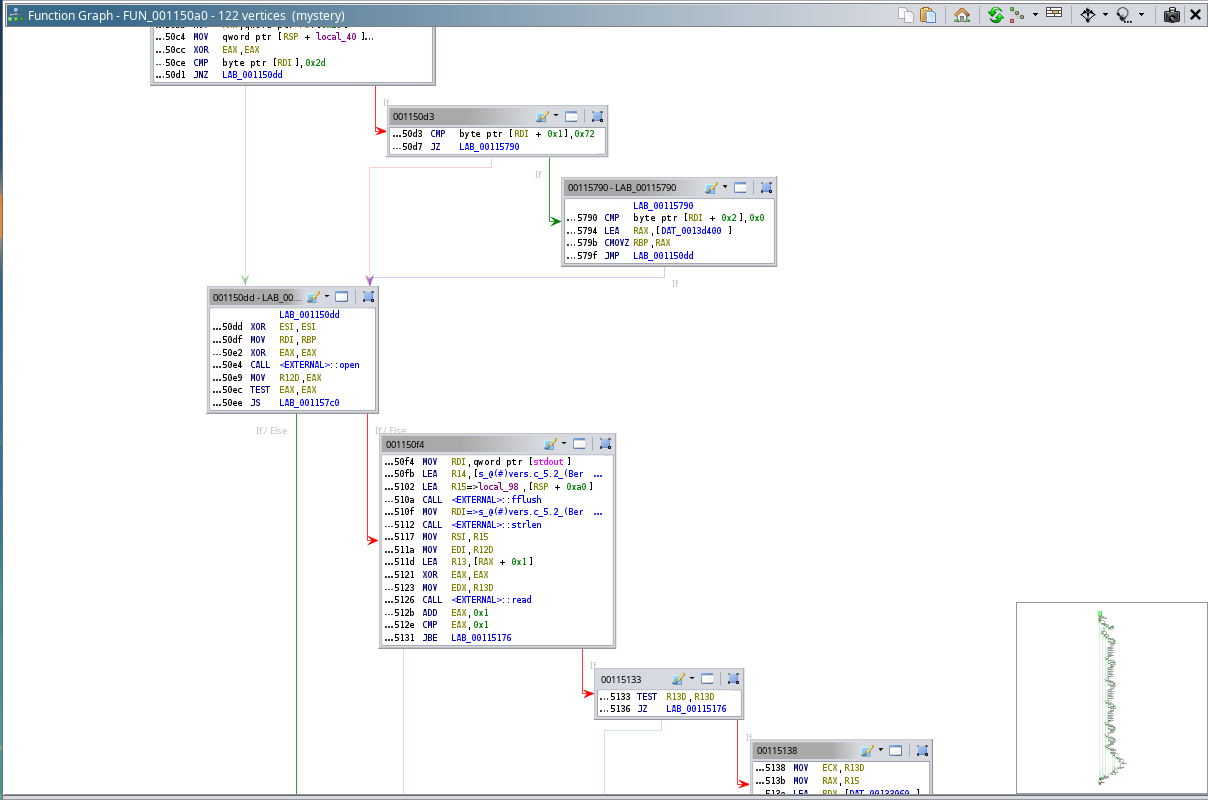
\includegraphics[height=0.95\textheight]{../re-tools/fun-graph-ex}
\end{frame}


\subsection{arrows on the side}
\begin{frame}{}
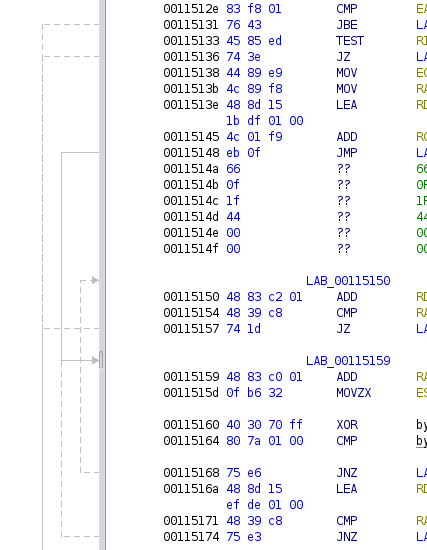
\includegraphics[height=0.9\textheight]{../re-tools/ghidra-side-arrows}
\end{frame}


\section{decompiling}

\subsection{decompiler}
\begin{frame}{decompiler}
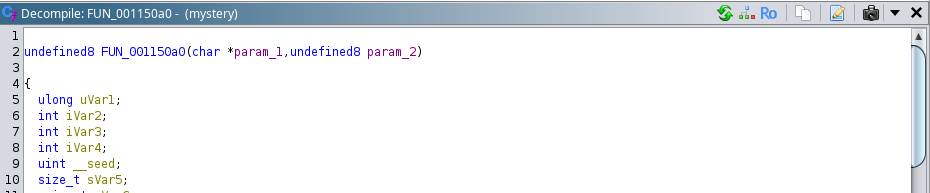
\includegraphics[width=0.9\textwidth]{../re-tools/decomp-top} \\
\ldots  \\
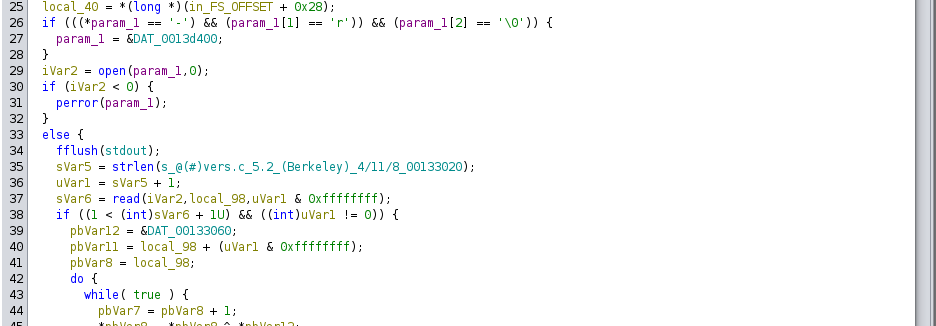
\includegraphics[width=0.9\textwidth]{../re-tools/decomp-rest}
\end{frame}

\begin{frame}{refining decompile (1)}
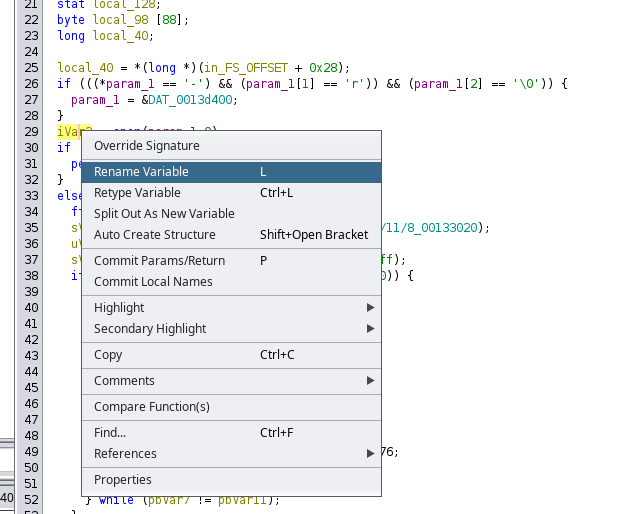
\includegraphics[width=0.9\textwidth]{../re-tools/ghidra-edit-var-decomp}
\end{frame}

\begin{frame}{refining decompile (2)}
    \begin{itemize}
    \item can setup names, types for functions
    \item types can include marking array
        \begin{itemize}
        \item Ghidra doesn't seem great at inferring this all the time
        \end{itemize}
    \vspace{.5cm}
    \item also for local/global variables
        \begin{itemize}
        \item for globals, can right-click in listing view too
        \end{itemize}
    \end{itemize}
\end{frame}



% intermediate representation for main() function in mystery
% decompiled representation
\subsection{Ghidra: intermediate representation}
\begin{frame}{interlude: editing disassembly format}
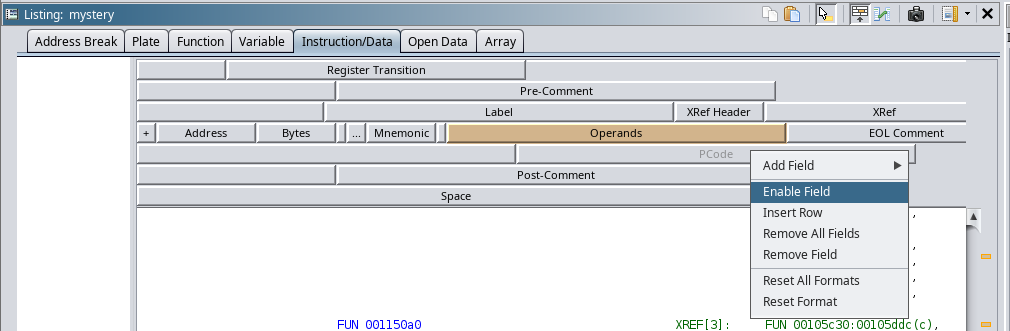
\includegraphics[width=\textwidth]{../re-tools/ghidra-enable-show-pcode}
\end{frame}

\begin{frame}{PCode}
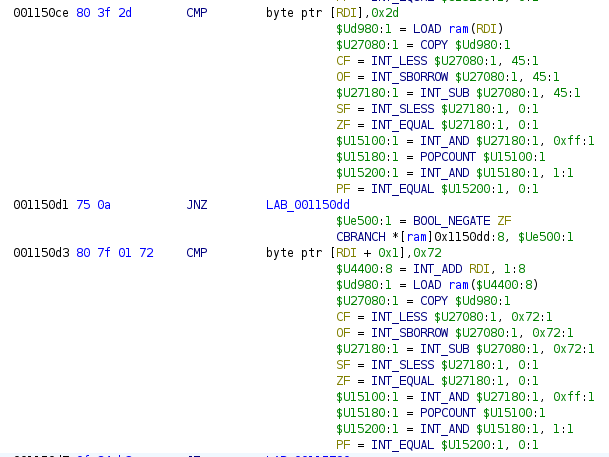
\includegraphics[height=0.9\textheight]{../re-tools/ghidra-pcode-ex}
\end{frame}

\begin{frame}{Intermediate Representations}
\begin{itemize}
\item Ghidra converts instructions to this PCode language
    \begin{itemize}
    \item describes effects of each instruction for other parts of Ghidra
    \item allows `easy' support for ARM, MIPS, \ldots
    \end{itemize}
\item function graph we saw using PCode information, probably
\item decompiler is basically a PCode to C compiler
    \begin{itemize}
    \item does the same kind of optimizations/etc. normal compiler does
    \item different output language
    \end{itemize}
\item Ghidra has `find similar functions' tool that probably uses this
\end{itemize}
\end{frame}




\section{more high-level overviews}

\subsection{data flow graphs}

\subsection{data type inference}

\section{annotate to improve}

\subsection{function naming}

\subsection{data, parameter types, arrays}

\section{patching things}
\begin{frame}{patch instruction?}
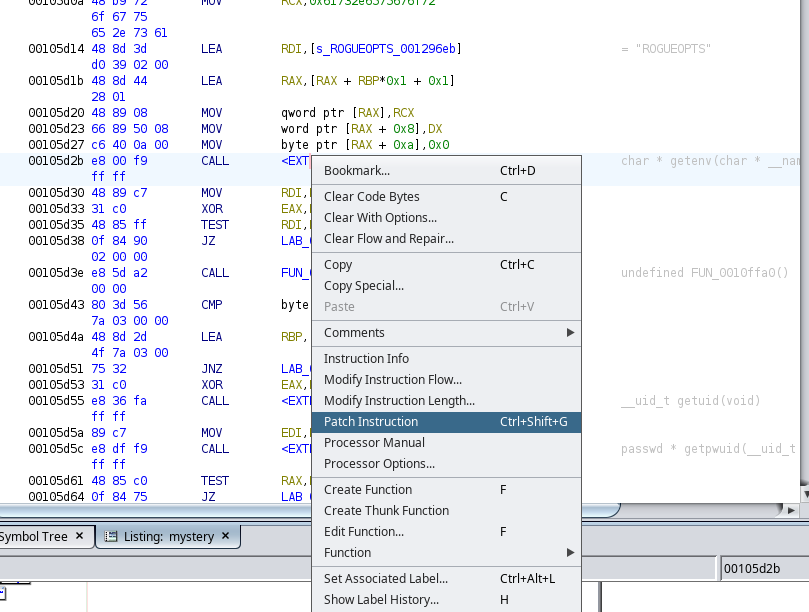
\includegraphics[width=\textwidth]{../re-tools/ghidra-patch-ex}
\end{frame}

\begin{frame}{patch instruction?}
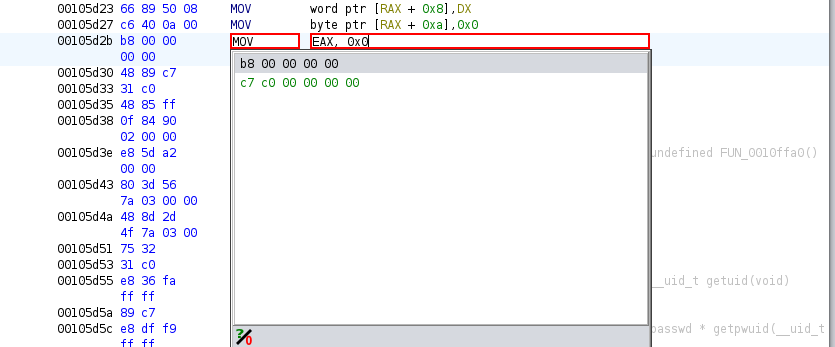
\includegraphics[width=\textwidth]{../re-tools/ghidra-patch-ex2}
\end{frame}

\begin{frame}{why is this useful?}
    \begin{itemize}
    \item can export modified version of binary to test
    \item ghidra has support for debugging or emulating running program
        \begin{itemize}
        \item emulation is another application of PCode representation
        \item debugging requires some work to configure
        \end{itemize}
    \end{itemize}
\end{frame}



\section{with debuggers}






\section{backup slides}
\begin{frame}{backup slides}
\end{frame}

\end{document}
